\pdfbookmark{Общая характеристика работы}{characteristic}             % Закладка pdf
\section*{Общая характеристика работы}

\newcommand{\actuality}{\pdfbookmark[1]{Актуальность}{actuality}\underline{\textbf{\actualityTXT}}}
\newcommand{\progress}{\pdfbookmark[1]{Разработанность темы}{progress}\underline{\textbf{\progressTXT}}}
\newcommand{\aim}{\pdfbookmark[1]{Цели}{aim}\underline{{\textbf\aimTXT}}}
\newcommand{\tasks}{\pdfbookmark[1]{Задачи}{tasks}\underline{\textbf{\tasksTXT}}}
\newcommand{\aimtasks}{\pdfbookmark[1]{Цели и задачи}{aimtasks}\aimtasksTXT}
\newcommand{\novelty}{\pdfbookmark[1]{Научная новизна}{novelty}\underline{\textbf{\noveltyTXT}}}
\newcommand{\influence}{\pdfbookmark[1]{Практическая значимость}{influence}\underline{\textbf{\influenceTXT}}}
\newcommand{\methods}{\pdfbookmark[1]{Методология и методы исследования}{methods}\underline{\textbf{\methodsTXT}}}
\newcommand{\defpositions}{\pdfbookmark[1]{Положения, выносимые на защиту}{defpositions}\underline{\textbf{\defpositionsTXT}}}
\newcommand{\reliability}{\pdfbookmark[1]{Достоверность}{reliability}\underline{\textbf{\reliabilityTXT}}}
\newcommand{\probation}{\pdfbookmark[1]{Апробация}{probation}\underline{\textbf{\probationTXT}}}
\newcommand{\contribution}{\pdfbookmark[1]{Личный вклад}{contribution}\underline{\textbf{\contributionTXT}}}
\newcommand{\publications}{\pdfbookmark[1]{Публикации}{publications}\underline{\textbf{\publicationsTXT}}}


{\actuality} 
Задачи оптимизации применяются в самых разных областях человеческой деятельности от экономики до машинного обучения. Например, методы оптимизации позволяют решать системы уравнений, моделировать экономические процессы, обучать нейросети и анализировать риски в банках. Такое многообразие приложений связано с тем, что задача оптимизации - это поиск лучшего доступного решения, которое удовлетворяет требованиям исследуемой модели. Методы оптимизации предлагают обширный выбор инструментов, которые распределены по характеристикам моделей и предъявляемых к ней ограничений. Общая постановка задачи минимизации имеет вид
$$
    \min_{x\in Q} {f\left( x \right)}.
$$
Здесь и всюду далее $n$ --- это размерность пространства переменных, а $Q$ --- выпуклое замкнутое подмножество $\mathbb{R}^n$. Учет размерности задачи в современном мире стал необходимостью, поскольку модели усложняются и количество учитываемых параметров растет экспоненциально. Подобный рост размерности привел к росту популярности численных методов оптимизации градиентного типа. Речь о методах, в которых на итерациях может использоваться информация о значении целевой функции ее градиента. К недостаткам данного типа методов можно отнести необходимость прибегать к информации о функциональных свойствах для исследуемых задач, таких как гладкость, липшицевость и сильная выпуклость. Напомним определения используемых далее функционального свойства. Одним из них является условие Липшица вида
$$
    |f(y) - f(x)| \leq M \norm{y-x}_2 \;\;\; \forall x, y \in Q
$$
при некотором фиксированном $M > 0$, а норма $\norm{\cdot}_2$ --- это евклидова норма. Гладкость целевой функции определяется как условие Липшица для градиента:
$$
    \norm{\nabla f(x) - \nabla f(y)}_2 \leq L \norm{x - y}_2 \;\;\; \forall x, y \in Q
$$
при некотором фиксированном $L > 0$.
Данное условие влечет неравенство, более часто применяемое на практике,
\begin{equation}\label{l_grad}
    f(y) \leq f(x) + \langle \nabla{f(x)}, y - x \rangle  + \frac{L}{2} \|x - y \|_2^2 \quad   \forall x, y \in Q.
\end{equation}
Часто полезным будет свойство сильной выпуклости функции \cite{Pol66}:
$$
\begin{aligned}
    f(\lambda x + &(1 - \lambda)y) \le\\ 
    &\lambda f(x) + (1 - \lambda)f(y) - \frac{\mu}{2} \lambda (1 - \lambda)\|x - y\|^2_2 \;\;\; \forall x, y \in Q,
\end{aligned}
$$
где $0 \le \lambda \le 1$, для некоторого $\mu > 0$, называемого константой сильной выпуклости.
Для таких функций верно неравенство
\begin{equation}
    f(x) + \langle \nabla f(x), y - x \rangle + \frac{\mu}{2} \norm{x - y}_2^2 \leq f(y) \;\;\; \forall x, y \in Q.
\end{equation}

Одна из причин популярности градиентных методов - это низкая затратность и возможность отказаться в оценках скорости сходимости от размерности задачи, что делает их применение эффективным для многих задач. В широком смысле под эффективностью метода оптимизации понимается время, необходимое для получения достаточно хорошего решения. Однако, подобная величина зависит от огромного количества аспектов, не имеющих прямого отношения к алгоритму поиска достаточно хорошего решения. Такими аспектами могут являться мощность вычислительного устройства, доступная точность представления чисел, необходимое количество памяти и т.д. Чтобы разделить технический и теоретический аспекты, под эффективностью численного метода оптимизации на определенном классе задач часто понимают именно эффективность в смысле Бахвалова-Немировского \cite{Nemirovski1979} --- число обращений по ходу работы метода к \textit{оракулу}, достаточное для достижения приемлемой точности. 
Оракулом называется подпрограмма расчета значений целевой функции (градиента, гессиана или некоторой заменяющей их величины) с необходимой точностью. Как правило, данное обращение является наиболее <<дорогостоящей>> частью шага. В некоторых ситуациях оптимизация работы оракула является необходимостью для приемлемой работы метода, этот аспект будет более подробно обсуждаться на примере в рамках 1й главы в пункте 1.3.5.

Таким образом, аналитическая сложность оптимизационной задачи для метода на заданном классе характеризуется количеством запросов к оракулу для гарантии нахождения приближенного решения с заранее заданной точностью $\varepsilon > 0$. Что можно более формально описать 
$$
    \norm{x_N - x_*}_2 \leq \varepsilon, 
$$
где $x_N$ --- точка выхода алгоритма после $N$ итераций используемого метода, а $x_*$ --- искомое точное решение задачи. Также часто рассматривают точность с точки зрения значения функции, а именно
$$
    |f(x_N) - f(x_*)| \leq \varepsilon.
$$

Оракульный подход очень удобен для анализа сложности и сравнения численных методов. Если ответы оракула являются локальными и не накладывают никаких ограничений, не требуют каких-либо свойств от исследуемой функции, то такой подход также называют \textit{концепцией чёрного ящика}.

Cуществует несколько типов оракульных оценок:
\begin{itemize}
    \item верхняя --- количество обращений к оракулу не более данного значения (хуже не будет),
    \item нижняя --- не менее данного числа обращений (лучше не будет),
    \item оптимальная соответствует ситуации, когда нижняя и верхняя оценки совпадают с точностью до константных множителей, не зависящих от параметров задачи, таких как размерность, константа гладкости и прочее.
\end{itemize}

Ранее многие задачи относились к задачам \textit{небольшой размерности}, но в последнее время размерность задач увеличивается. Задачей \textit{небольшой размерности} обычно называют задачу, когда возможно $N \geq n$, где $N$ --- количество обращений к оракулу, а $n$ --- размерность пространства. На практике к задачам небольшой размерности можно отнести задачи, имеющие размерность в несколько сотен. Неплохую эффективность для таких задач имеют методы секущей гиперплоскости, к которым относятся метод центров тяжести и метод эллипсоидов. Однако их оптимальные оценки $N \sim \mathcal{O}\left(n \log{n}\right)$ существенно зависят от размерности пространства \cite{bubeck_2015}. 
Эта зависимость приводит к высоким требованиям по необходимой памяти и необходимости увеличения количества итераций с ростом размерности пространства для сохранения той же точности. Градиентные методы в противоположность им обладают сравнительно скромными требованиями по необходимой памяти, и соответствующие оценки не зависят от размерности задачи. Отметим также, что лучшие верхние оценки на классе гладких выпуклых функций известны для ускоренных методов \cite{Nesterov1983}.

Как уже было отмечено ранее, недостатком данного типа методов является необходимость ряда функциональных свойств у исследуемой функции. Выпишем известные оптимальные оценки сложности задач выпуклой оптимизации в зависимости от предположений о гладкости задачи.

\begin{table}[h]
    \caption{Оптимальные оценки количества обращений к субградиенту.}
    \label{est_tbl}
    \centering
    \begin{tabular}{|c|c|c|}
        \hline
         & \makecell{$|f(y) - f(x)| \leq$ \\ $\leq M \| y - x \|_2$} & \makecell{$\|\nabla f(y) - \nabla f(x)\|_2 \leq $\\ $\leq L \| y - x \|_2$} \\
        \hline
        $f(x)$ -- выпукла & $\mathcal{O} \left( \frac{M^2 R^2}{\varepsilon^2} \right)$ & $\mathcal{O} \left( \sqrt{\frac{L R^2}{\varepsilon}} \right)$ \\
        \hline
        \makecell{$f(x)$ -- $\mu$-сильно \\ выпукла в $\| \cdot \|_2$ - норме} & $\mathcal{O} \left( \frac{M^2}{\mu \varepsilon} \right)$ & $\mathcal{O} \left( \sqrt{\frac{L}{\mu}} \left[\ln{\frac{\mu R^2}{\varepsilon}}\right] \right)$ \\
        \hline
    \end{tabular}
\end{table}
В таблице \ref{est_tbl} $R$ --- это $\|x_0 - x_*\|_2 $, а $x_0$ --- стартовая точка алгоритма. Как видим, оценки в гладком случае существенно лучше, чем в негладком. В случаях, когда функционалы не обладают достаточными свойствами гладкости, что проявляется во многих задачах, актуальны вопросы разработки соответствующих эффективных методов. Для негладких задач нет возможности гарантировать высокую скорость сходимости. В данной работе рассматриваются некоторые типы негладких задач для которых исследуются возможные усовершенствования известных результатов при дополнительных условиях. Важным направлением является исследование обобщений уже известных классов задач, которые позволяют сохранить приемлемые вычислительные гарантии сходимости численных методов.

\iffalse
    Для улучшения оценок для негладких задач существует несколько подходов. Например, выделяют специальные подклассы задач, при помощи, например, условия острого минимума, предложенного в конце 1960-х годов Б.Т. Поляком \cite{Polyak1969}. Стоит подчеркнуть, что подобные условия зачастую выставляют более жесткие требования к задаче. 
\fi

Напомним, что для негладких задач в качестве обобщения понятия градиента рассматривают понятие субградиента. Вектор $g$ называют субградиентом в точке $x_0$, если
$$
    f(x) \geq f(x_0) + \langle g, x - x_0 \rangle \;\;\; \forall x \in Q.
$$

Известно, что оптимальная оценка субградиентного метода сублинейна на классах как выпуклых, так и сильно выпуклых липшицевых задач \cite{Bach_2012}. Это трудно считать достаточным для ряда приложений. В связи с этим для улучшения оценок скорости сходимости субградиентных методов используют такие допущения, как, например, условие острого минимума. Некоторые новые результаты в этом направлении изложены в данной работе.
\iffalse
    Подобные условия позволяют сделать несколько начальных эффективных шагов, что было продемонстрировано в работе \cite{sharp22} и будет затронуто во второй главе данной работы. Также в упомянутой главе было проведено сравнение оценок скорости субградиентных для классов задач с острым минимумом и сильной выпуклостью. Острый минимум может приводить к лучшей оценке скорости сходимости, однако данное свойство требует информации о точном решении, что является существенным ограничением.

    Оценки, получаемые при помощи условия острого минимума, обладают лучшими свойствами сходимости, однако в отсутствии знаний о точном решении нет возможности повысить точность выше предварительно заданной точности, известной для приближенного решения. Оценки скорости сходимости, использующие сильную выпуклость, не обладают столь впечатляющими оценками скорости сходимости, однако позволяют добиться гораздо большей точности. 
\fi

Отметим важное и развиваемое в данной работе обобщение оптимальных результатов для субградиентного метода на случай задачи с аналогом условия Липшица относительно некоторой выпуклой прокс-функции (относительная липшицевость). Такая прокс-функция, в отличие от классической постановки, не обязана удовлетворять условию сильной выпуклости относительно нормы \cite{AdaMirr_2021,Lu_2018,Zhou_NIPS_2020}. Напомним важное понятие дивергенции (расхождения) Брэгмана. Предполагается, что нам доступна некоторая выпуклая (вообще говоря, не сильно выпуклая) дифференцируемая прокс-функция $d$, порождающая некоторое расстояние, и соответствующая ей дивергенция (расхождение) Брэгмана \cite{Bauschke}
\[
    V(y, x) = d(y) - d(x) - \langle \nabla d(x), y - x \rangle.
\]

При помощи дивергенции Брэгмана вводятся такие необходимые понятия, как \textit{относительная липишицевость, относительная сильная выпуклость, относительная гладкость и условие относительного $\gamma$-роста}. Например, свойство относительной $L$-гладкости функции $f$ обобщает условие $L$-гладкости $f$ (см. \eqref{l_grad}), где квадрат евклидовой нормы в определении заменяется дивергенцией Брэгмана
$$
    f(y) \leq f(x) + \langle \nabla{f(x)}, y - x \rangle  + L V(y,x) \quad   \forall x, y \in Q,
$$
где $Q$ --- область определения $f$.

Наиболее заметными современными приложениями, обладающими свойствами относительной гладкости и относительной сильной выпуклости, являются задачи распределенной оптимизации в предположении схожести слагаемых \cite{Hendr}. 

Во второй главе данной работы исследуется оценка скорости сходимости субградиентного метода для сильно выпуклых задач с аналогичным предположением об относительной липшицевости. Точнее, рассматривается вариант субградиентного метода на классе относительно ограниченных и относительно сильно монотонных вариационных неравенств, а также класс относительно сильно выпукло-вогнутых седловых задач с соответствующими условиями относительной липшицевости функционалов. Вариационные неравенства являются важной вехой для работы, например, с лагранжевыми седловыми задачами. Известно, что задача решения вариационного неравенства имеет вид
$$
    \max_{x \in Q} \langle g(x), x_* - x \rangle \leq 0,
$$
где $x_*$ называют слабым решением вариационного неравенства, $Q$ --- выпуклое замкнутое подмножество $\mathbb{R}^n$, $g: Q \longrightarrow \mathbb{R}^n$. Предполагается, что решение $x_*$ существует. Такая постановка приводит к существенно более широкому классу задач, чем минимизационные задачи. Класс вариационных неравенств имеет достаточно широкую область применения в различных областях математики, таких как теория игр, моделирование потоков и математическая экономика. 

В третьей главе вводится понятие относительного $\gamma$-роста целевой функции, которое позволяет улучшить сублинейные оценки скорости сходимости субградиентного метода (зеркального спуска в случае неевклидовой прокс-структуры) для сильно выпуклых функций при помощи рестартов оригинального метода. Предлагается удобный с практической точки зрения алгоритм, использующий адаптивный критерий остановки на каждом из рестартов. 

% {\progress}
% Этот раздел должен быть отдельным структурным элементом по
% ГОСТ, но он, как правило, включается в описание актуальности
% темы. Нужен он отдельным структурынм элемементом или нет ---
% смотрите другие диссертации вашего совета, скорее всего не нужен.

{\aim} данной работы является развитие теории методов оптимизации для задач, не обладающих стандартными условиями гладкости, с упором на анализ субградиентных методов на классе задач с современными аналогами условий Липшица, сильной выпуклости и $\gamma$-роста ($\gamma > 1$).

{\underline{\textbf{Задачи,}}} решаемые в данной диссертации:
\begin{enumerate}
    \item Экспериментальная проверка теоретических результатов для задач распределенной оптимизации, не обладающая стандартными условиями гладкости, недавно полученных соавторами в работе \cite{GorbunovKMR20}.
    \item Экспериментальный анализ методов безградиентного, градиентного и квазинютоновского типов для работы с невыпуклым, вообще говоря, функционалом специальной структуры, а именно практический анализ возможностей эффективной оптимизации для задачи минимизации белка, имеющей различные физические основания,  OPLS force field. 
    \item Вывод оценки скорости сходимости зеркального спуска с использованием адаптивно подбираемых параметров на классе сильно выпуклых задач. Доказательство оценки скорости сходимости зеркального спуска для относительно ограниченных и относительно сильно монотонных операторов на классе вариационных неравенств.
    \item Исследование специальной методики рестартов зеркального спуска для относительно липшицевых задач минимизации с условием относительного $\gamma$-роста. 
\end{enumerate}
В данной работе мы для метода зеркального спуска рассматриваем аналоги условия Липшица, которые позволяют сохранить свойственные липшицевым задачам оптимальные оценки скорости сходимости. Также производится переход к аналогичной постановке задачи в терминах вариационных неравенств, что позволяет дополнительно расширить доступный класс задач. Получены улучшенные оценки скорости сходимости при помощи механизма рестартов зеркального спуска в случае наличия дополнительных условий острого минимума или относительного $\gamma$-роста. Сделан существенный акцент на экспериментальной составляющей.

{\novelty}
\begin{enumerate}[beginpenalty=10000] % https://tex.stackexchange.com/a/476052/104425
  \item Впервые получены оценки скорости сходимости метода зеркального спуска на классе вариационных неравенств с относительно сильно монотонными и относительно ограниченными операторами.
  \item Впервые получен адаптивный аналог оптимальной оценки скорости сходимости зеркального спуска для задач минимизации сильно выпуклых функций с использованием локальных аналогов константы Липшица.
  \item Впервые получены оценки скорости сходимости рестартованного метода зеркального спуска для относительно липшицевых задач оптимизации с относительным $\gamma$-ростом при $\gamma > 1$. 
\end{enumerate}

{\defpositions}
\begin{enumerate}[beginpenalty=10000] % https://tex.stackexchange.com/a/476052/104425
  \item Предложен вариант метода зеркального спуска для вариационных неравенств с относительно сильно монотонными и относительно ограниченными операторами. Доказана инвариантная по размерности пространства оценка скорости сходимости этого метода, оптимальная на указанном классе задач с точностью до умножения на постоянный множитель.
  \item Получена адаптивная оценка скорости сходимости зеркального спуска для задач минимизации сильно выпуклых функций с использованием локальных аналогов константы Липшица. При этом сохраняется оптимальность этой оценки на классе сильно выпуклых липшицевых задач с точностью до умножения на константу. В частности, это позволяет работать и с задачами, не удовлетворяющими условию Липшица.
  \item Введён аналог острого минимума ($\gamma$-роста) с использованием дивергенции Брэгмана. Получена оценка скорости сходимости рестартованного метода зеркального спуска для относительно липшицевых задач оптимизации с относительным $\gamma$-ростом. В ситуации сильно выпуклой прокс-функции предложены адаптивные правила остановки для рестартов исследуемого метода зеркального спуска и получен результат о его скорости сходимости.
\end{enumerate}

{\probation}
Основные результаты работы докладывались~на:
\begin{itemize}
    \item проектной смене <<Современные методы теории информации, оптимизации и управления>> в центре <<Сириус>>, 2021,
    \item QIPA (Quasilinear Equations, Inverse Problems and Their Applications), 2021,
    \item 64-й всероссийской научной конференции МФТИ, 2021,
    \item QIPA (Quasilinear Equations, Inverse Problems and Their Applications), 2018,
    \item 61-й всероссийской научной конференции МФТИ, 2018.
\end{itemize}

{\contribution} Ключевые результаты получены и доказаны автором лично. Также разработана библиотека для анализа и проверки методов оптимизации, обеспечивающая необходимую гибкость настройки. 

\ifnumequal{\value{bibliosel}}{0}
{%%% Встроенная реализация с загрузкой файла через движок bibtex8. (При желании, внутри можно использовать обычные ссылки, наподобие `\cite{vakbib1,vakbib2}`).
    {\publications} Основные результаты по теме диссертации изложены
    в~XX~публикациях,
    X из которых изданы в журналах, рекомендованных ВАК,
    X "--- в тезисах докладов.
}%
{%%% Реализация пакетом biblatex через движок biber
    \begin{refsection}[bl-author, bl-registered]
        % Это refsection=1.
        % Процитированные здесь работы:
        %  * подсчитываются, для автоматического составления фразы "Основные результаты ..."
        %  * попадают в авторскую библиографию, при usefootcite==0 и стиле `\insertbiblioauthor` или `\insertbiblioauthorgrouped`
        %  * нумеруются там в зависимости от порядка команд `\printbibliography` в этом разделе.
        %  * при использовании `\insertbiblioauthorgrouped`, порядок команд `\printbibliography` в нём должен быть тем же (см. biblio/biblatex.tex)
        %
        % Невидимый библиографический список для подсчёта количества публикаций:
        \printbibliography[heading=nobibheading, section=1, env=countauthorvak,          keyword=biblioauthorvak]%
        \printbibliography[heading=nobibheading, section=1, env=countauthorwos,          keyword=biblioauthorwos]%
        \printbibliography[heading=nobibheading, section=1, env=countauthorscopus,       keyword=biblioauthorscopus]%
        \printbibliography[heading=nobibheading, section=1, env=countauthorconf,         keyword=biblioauthorconf]%
        \printbibliography[heading=nobibheading, section=1, env=countauthorother,        keyword=biblioauthorother]%
        \printbibliography[heading=nobibheading, section=1, env=countregistered,         keyword=biblioregistered]%
        \printbibliography[heading=nobibheading, section=1, env=countauthorpatent,       keyword=biblioauthorpatent]%
        \printbibliography[heading=nobibheading, section=1, env=countauthorprogram,      keyword=biblioauthorprogram]%
        \printbibliography[heading=nobibheading, section=1, env=countauthor,             keyword=biblioauthor]%
        \printbibliography[heading=nobibheading, section=1, env=countauthorvakscopuswos, filter=vakscopuswos]%
        \printbibliography[heading=nobibheading, section=1, env=countauthorscopuswos,    filter=scopuswos]%
        %
        \nocite{*}%
        %
        {\publications} Основные результаты по теме диссертации изложены в~\arabic{citeauthor}~печатных изданиях
        % \arabic{citeauthorvak} из которых изданы в журналах, рекомендованных ВАК\sloppy% 
        \ifnum \value{citeauthorscopuswos}>0%
            , \arabic{citeauthorscopuswos} "--- в~периодических научных журналах, индексируемых Web of~Science или Scopus\sloppy%
        \fi%
        \ifnum \value{citeauthorconf}>0%
            , \arabic{citeauthorconf} "--- в~тезисах докладов.
        \else%
            .
        \fi%
        \ifnum \value{citeregistered}=1%
            \ifnum \value{citeauthorpatent}=1%
                Зарегистрирован \arabic{citeauthorpatent} патент.
            \fi%
            \ifnum \value{citeauthorprogram}=1%
                Зарегистрирована \arabic{citeauthorprogram} программа для ЭВМ.
            \fi%
        \fi%
        \ifnum \value{citeregistered}>1%
            Зарегистрированы\ %
            \ifnum \value{citeauthorpatent}>0%
            \formbytotal{citeauthorpatent}{патент}{}{а}{}\sloppy%
            \ifnum \value{citeauthorprogram}=0 . \else \ и~\fi%
            \fi%
            \ifnum \value{citeauthorprogram}>0%
            \formbytotal{citeauthorprogram}{программ}{а}{ы}{} для ЭВМ.
            \fi%
        \fi%
        % К публикациям, в которых излагаются основные научные результаты диссертации на соискание учёной
        % степени, в рецензируемых изданиях приравниваются патенты на изобретения, патенты (свидетельства) на
        % полезную модель, патенты на промышленный образец, патенты на селекционные достижения, свидетельства
        % на программу для электронных вычислительных машин, базу данных, топологию интегральных микросхем,
        % зарегистрированные в установленном порядке.(в ред. Постановления Правительства РФ от 21.04.2016 N 335)
    \end{refsection}%
    \begin{refsection}[bl-author, bl-registered]
        % Это refsection=2.
        % Процитированные здесь работы:
        %  * попадают в авторскую библиографию, при usefootcite==0 и стиле `\insertbiblioauthorimportant`.
        %  * ни на что не влияют в противном случае

        % \nocite{vakbib2}%vak
        % \nocite{patbib1}%patent
        % \nocite{progbib1}%program
        % \nocite{bib1}%other
        % \nocite{confbib1}%conf
    \end{refsection}%
        %
        % Всё, что вне этих двух refsection, это refsection=0,
        %  * для диссертации - это нормальные ссылки, попадающие в обычную библиографию
        %  * для автореферата:
        %     * при usefootcite==0, ссылка корректно сработает только для источника из `external.bib`. Для своих работ --- напечатает "[0]" (и даже Warning не вылезет).
        %     * при usefootcite==1, ссылка сработает нормально. В авторской библиографии будут только процитированные в refsection=0 работы.
}

% \ifsynopsis
% \else
%   \insertbiblioauthor      % Вывод всех работ автора
% \fi
 % Характеристика работы по структуре во введении и в автореферате не отличается (ГОСТ Р 7.0.11, пункты 5.3.1 и 9.2.1), потому её загружаем из одного и того же внешнего файла, предварительно задав форму выделения некоторым параметрам

%Диссертационная работа была выполнена при поддержке грантов \dots

%\underline{\textbf{Объем и структура работы.}} Диссертация состоит из~введения,
%четырех глав, заключения и~приложения. Полный объем диссертации
%\textbf{ХХХ}~страниц текста с~\textbf{ХХ}~рисунками и~5~таблицами. Список
%литературы содержит \textbf{ХХX}~наименование.

\pdfbookmark{Содержание работы}{description}                          % Закладка pdf
\section*{Содержание работы}
Во \underline{\textbf{введении}} обоснована актуальность диссертационной работы, сформулирована цель и аргументирована научная новизна исследований и представлены выносимые на защиту положения. Описываются распространенные постановки задачи минимизации, вводится понятие оракульной сложности, упоминаются возможные несоответствия между практическим временем работы и получаемой оценкой. Также описываются причины, благодаря которым сейчас наиболее популярны методы градиентного типа. 

\underline{\textbf{Первая глава}} посвящена обзору литературы по теме выпуклой оптимизации. Описываются различные постановки задачи минимизации и ряд известных методов, широко использующихся на практике. Описываются классические градиентные методы и адаптивные квазиньютоновские. Описывается пример постановки и работы с задачей распределенной оптимизации, а также со специальной функцией, не обладающей выпуклостью, описывающей энергию молекулы белка. В качестве иллюстрации приводится опыт работы с нестандартным невыпуклым функционалом, для которого нет хороших вычислительных гарантий, что позволяет применить методы нулевого порядка и провести некоторый технический анализ.

\underline{\textbf{В параграфе 1.1}} приводится обзор методов первого порядка. Вводится общая постановка задачи, приводятся оптимальные оценки важных классов задач. Также рассматриваются популярные постановки задач, например задача минимизации квадратичной формы. Проводятся пояснения о стандартных способах улучшения оценок скорости сходимости для методов, таких как механизм рестартов, который в дальнейшем будет использован в 3й главе. Упоминаются ограничения и <<тонкие>> места, возникающие при работе с квазиньютоновскими методами, что имеет существенное значение в анализе задачи минимизации энергии белка. Многие из представленных в данной главе методов будут использованы для анализа функционала упомянутой задачи.

\underline{\textbf{Параграф 1.2}} описывает постановку задачи для распределенной минимизации
  \begin{equation} \label{raspr_task}
    \min_{x \in \mathbb{R}^n}\left\{f(x)=\frac{1}{d} \sum_{i=1}^d f_i(x)\right\},
  \end{equation}
  где $d$ соответствует количеству исполнителей или узлов или вычислителей. 

  Во введении уже обсуждалась связь эффективности применения метода и используемого исполнительного устройства или топологии устройств. В связи с ростом популярности машинного обучения и значительного времени, которое требуется для обучения современных моделей (дни, недели), задачи параллелизации и распределения исполнения по различным устройствам для эффективного их использования выходят на первый план.

  Будем предполагать, что информация, касающаяся функции $f_i$, хранится только на узле $i$. Также зачастую каждую из $f_i$ рассматривают как
  $$
    f_i(x) = \frac{1}{m} \sum_{j=1}^m f_{ij}(x).
  $$ 
  Значимым параметром, влияющим на скорость сходимости, является дороговизна пересылки информации между узлами. Данный аспект является так называемым бутылочным горлышком для подобного типа задач. Потому методы, нацеленные на распределенную постановку, как правило, стараются заменить глобальный шаг (обновление всех компонент вектора $x$) на локальные аналоги. Это основная идея, которая лежит в основе таких методов как Local-SGD \cite{Stich2019LocalSC}. Также популярным подходом является уменьшение передаваемой информации между узлами путем выбора наиболее значимых компонент или более сложных механизмов компрессии. Подобные подходы используются в работах \cite{qlsgd, qsgd, err_fdbk}. Отметим, что многие методы предполагают полносвязную топологию доступных узлов или же star-топологию, когда есть один вычисляющий центр и зависимые дополнительные мощности. 
  В работе \cite{GorbunovKMR20}, например, предлагается следующий метод
  $$
  \begin{aligned} 
    x^{k+1} &=x^k-\frac{1}{d} \sum_{i=1}^d v_i^k, \\ 
    e_i^{k+1} &=e_i^k + \gamma g_i^k - v_i^k, \quad i=1,2, \ldots, d . 
  \end{aligned}
  $$
  Здесь $x^k$ отвечает за значение аргумента на итерации $k$, $v_i^k$ --- это результат вычисленный на узле $i$ на итерации $k$, $g_i^k$ --- это оценка $\nabla f_i(x^k)$ полученная узлом $i$, $\gamma$ --- это фиксированный размер шага и $e_i^k$ --- это накопленная к итерации $k$ на узле $i$ ошибка.  Подобная постановка задачи рассматривалась также и в \cite{err_fdbk}, где был проведен схожий анализ, но со своими особенностями, учитывающий отложенное вычисление градиента, компрессию и размеры обновляемой части градиента.
  В упомянутой работе функция компрессии $C()$ представлена так:
  $$
    v_i^k = C(e_i^k + \gamma g_i^k).
  $$
  Данная постановка, как и было показано в \cite{GorbunovKMR20} моими соавторами, обобщает и развивает ряд методов, таких как Error Compensated Stochastic Gradiend Descent (EC-SGD), EC-SGD-DIANA и EC-LSVRG. Теоретические результаты для данного ряда методов также были получены моими соавторами. Однако многие практические результаты были получены автором. В упомянутой статье рассматривается задача линейной регрессии для различных наборов данных
  $$
    \min_{x \in \mathbb{R}^n}\left\{ f(x) = \frac{1}{N} \sum_{i=1}^N \log \left(1+\exp \left(- y_i \cdot(A x)_i\right)\right) + \frac{\mu}{2}\|x\|^2 \right\},
  $$
  где $N$ --- это количество параметров модели, $x$ --- это веса модели, $A$ --- матрица параметров, а $y \in {\{-1,1\}}^N$ --- набор ожидаемых решений. Подобный тип задач имеет широкое распространение в машинном обучении. Важным аспектом являются используемые функции компрессии, а именно 
  \begin{enumerate}
    \item функция $TopK()$ --- $k$ компонентов, отсортированных по убыванию абсолютных значений в векторе ошибок $e_i$,
    \item $RandK()$ --- $k$ случайных компонентов,
    \item $l2-quant()$ --- выделение некоторого подпространства в $\mathbb{R}^n$ на основе вероятности, полученной при помощи нормализации входного вектора. 
  \end{enumerate}

  Очевидно, что подобные преобразования понижают допустимую точность для методов и также появляется шум, связанный с компрессией. Поскольку здесь присутствует достаточно много параметров, которые варьируются для многих методов и различных функций компрессии, то мы приведем один из тестов в качестве иллюстрации влияния компрессии на различные методы --- см. рис. \ref{compr}. Здесь mushrooms --- это наименование использованного набора данных, по горизонтальной оси отложено количество итераций. Видно, что различные методы реагируют на внедрение функции компрессии по-разному. Некоторое методы более устойчивы к компрессионному шуму и позволяют эффективно повышать точность с ростом количества итераций, а именно EC-L-SVRG-DIANA.
  \begin{figure}
    \begin{center}
      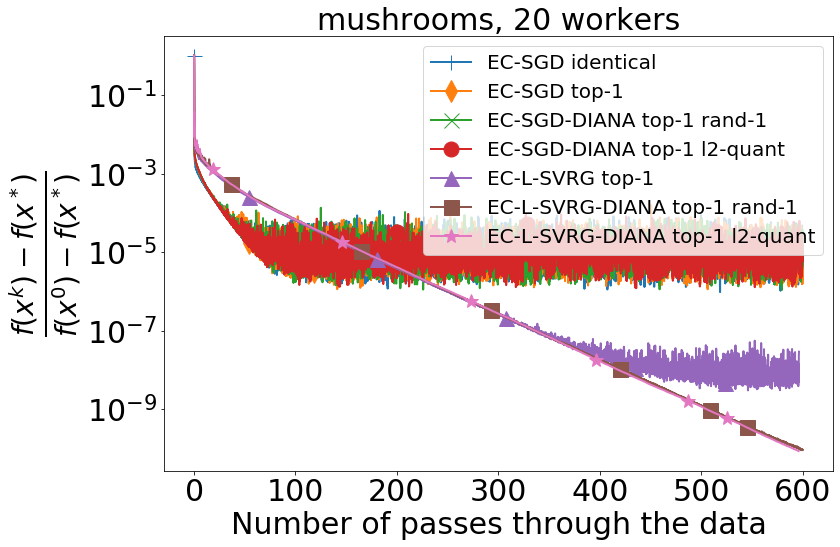
\includegraphics[height=0.24\paperheight]{mushrooms_20.png}
    \end{center}
    \caption{Компрессионный шум для различных методов.}
    \label{compr}
  \end{figure}
  В ряде задач требуется сочетания подходов, применяемых для распределенной оптимизации, и методов, использующих свойство относительной гладкости \cite{distrib_relative}. 

  К примеру, если в исходной постановке задачи распределенной оптимизации \eqref{raspr_task} $f_{ij}(x)$ являются $\mu$-сильно выпуклыми в 2-норме гладкими функциями, то можно предложить следующий дизайн градиентного спуска. Предположим, что есть централизованная архитектура с $d \ll m$ узлами. Первый узел является центральным. Это также называют star-топологией. Поместим в первый узел случайно отобранные $\tilde{m}(\widetilde{m} \ll m)$ слагаемых из суммы. Остальные слагаемые распределим по остальным узлам. Обозначим соответствующую первому узлу нормированную подсумму через $\widetilde{f_0}(x)$. Рассмотрим градиентный спуск, выполняемый на центральном узле $(k=0,1,2, \ldots)$ :
  $$
    x^{k+1}=\underset{x \in \mathbb{R}^n}{\arg \min }\left\{\left\langle\nabla f_0\left(x^k\right), x - x^k\right\rangle+L V\left(x, x^k\right)\right\},
  $$
  где
  $$
    V(y, x)=d(y)-d(x)-\langle\nabla d(x), y-x\rangle,\;\;\;d(x)=\widetilde{f_0}(x)+\frac{\gamma}{2}\|x\|_2^2, \;\;\; \gamma>0 .
  $$
  Каждая итерация такого градиентного спуска должна отвечать коммуникации центрального узла с остальными, чтобы в итоге получилось $\nabla f\left(x^k\right)$.
  С использованием результатов для градиентного метода на классе относительно гладких и относительно сильно выпуклых задач известна следующая оценка скорости сходимости
  $$
    f(\hat{x})-f_* \leqslant V\left(x_*, x^0\right)\left(1-\frac{\mu}{\mu+2 \gamma}\right)^N.
  $$
  Это интересно при $\gamma << L$. Аккуратное доказательство для градиентного спуска в схожей постановке представлено в \cite{distrib_relative}.

\underline{\textbf{Параграф 1.3}} содержит анализ и предпринятые шаги по работе с практической задачей, возникшей в области вычислительной биологии. Приводится опыт работы с функционалом, не обладающим достаточной выпуклостью и основанным на ряде физических свойств объекта (что показано на рис. \ref{fig1D}). 

\begin{figure}
\begin{center}
    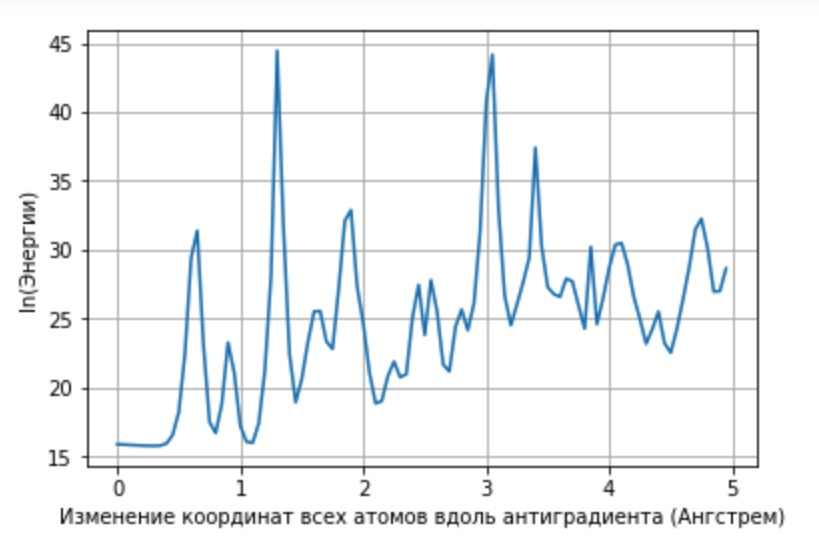
\includegraphics[height=0.24\paperheight]{1DSearch.jpg}
\end{center}
\caption{Отсутствие выпуклости задачи минимизации OPLS force field}
\label{fig1D}
\end{figure}
     
Сам пункт имеет разбиение на ряд подпунктов которые отвечают за различные этапы анализа и работы с задачей. В первом подпункте 1.3.1 описывается проблематика задачи и мотивация для ее решения. Данная задача относится к типу задач большой размерности:  $n_{ }\left(n\sim 10^4\right)$. 

Второй подпункт 1.3.2 описывает физические основания, стоящие за структурой функционала. Энергия белка основана на взаиморасположении атомов в молекуле и их различных взаимодействиях. Каждый атом в данном случае описывается тремя пространственными координатами, а самый простой белок состоит из $100$ атомов. Что позволяет оценить размерность пространства возможных конфигураций молекулы. Для подобного функционала вычисление градиента является весьма трудоемкой задачей, что объясняется сложностью и большим количеством параметров. Выпуклость пропадает в силу специфики ряда физических взаимодействий. Также стоит отметить, что в задаче необходимо найти ближайший устойчивый локальный минимум, поскольку в естественных условиях стремление к глобальному минимуму отсутствует. 

Третий пункт 1.3.3 описывает обсуждения и мотивацию, стоящую за выбором методов. Оптимизируемый функционал может рассматриваться как гладкий только локально. Константа Липшица не является равномерно ограниченной в достаточно большой окрестности точки старта. Но в таком случае для минимизации такого функционала нет гарантий даже локальной сходимости \cite{ghadimi2015generalized}, \cite{nesterov2017random}.
   
Для решения таких задач глобальной оптимизации теория рекомендует использовать безградиентные методы типа simulated annealing или марковского поиска \cite{zhigljavsky2007stochastic}, \cite{zhigljavsky2012theory}.
Были проведены эксперименты с методами нулевого порядка (покоординатный спуск в различных вариациях). В основе предлагаемого подхода -- <<шевеление>> на каждой итерации только одного, случайно выбранного, атома при <<замороженных>> остальных. Заметим, что при изменении положения одного атома пересчет некоторых частей функционала будет стоить $\mathcal{O}\left( 1 \right)$ с точки зрения сложности вычислений, поскольку затрагивает только <<соседние>> по химическим связям атомы. Здесь под <<соседними>> имеются в виду не только непосредственные соседи, но и соседи через две и даже три химические связи. Обычно число таких соседей не больше 15. 

Поскольку задача является практической основным приоритетом было качество и скорость работы используемого метода. В итоге возникло интересное противопоставление - безградиентного метода со значительной параллелизацией и более линейного метода сопряженных градиентов. Однако во время работы с покоординатным спуском было обнаружено, что можно получить значительное ускорение при использовании гладкости вдоль каждой из координатных осей. Это было одним из сигналов, что градиентные методы могут быть успешно применены и для данной задачи. Эксперименты это и подтвердили, как итог финальная реализация основывалась на методах сопряженных градиентов.

\begin{table}[h]
\caption{Сравнение характеристик методов}
\label{tabular:timesandtenses}
\centering
\resizebox{\textwidth}{!}{
    \begin{tabular}{|c|c|c|}
        \hline
        \fontsize{12pt}{12pt}\selectfont {\bfseries Показатели} & {\bfseries <<Шевеление>> атома} & {\bfseries Адаптивный градиентный спуск} \\
        \hline
        \fontsize{12pt}{12pt}\selectfont Время 1 итерации, секунды    & 1.2075 & 122.9814 \\
        \hline
        \fontsize{12pt}{12pt}\selectfont Энергия 1 итерации, кДж/моль & 0.0225 & 2.7081 \\
        \hline
        \fontsize{12pt}{12pt}\selectfont $\sim\Delta$Энергии к 300 минуте, кДж/моль & $- 347$ & $- 413$ \\
        \hline
    \end{tabular}
}
\end{table}

Пункт 1.3.4 и 1.3.5 содержат детали реализации и описание проблем, возникших во время работы. Более подробно описываются модификации квазиньютоновских методов и методы одномерного поиска, адаптированные к структуре задачи.

Пункт 1.3.6 описывает результаты экспериментов, как оценивалось качество полученных решений и какие дополнительные параметры рассматривались. Ускоренный градиентный спуск и метод сопряженных градиентов показали лучшие результаты на тестовых наборах данных. Однако, отметим, что для получения данных результатов пришлось ввести ряд поправок для соответствия структуре задаче. 

\underline{\textbf{Во второй главе}} представлено исследование методов первого порядка для ряда классов вариационных неравенств с операторами, удовлетворяющими предлагаемому аналогу условия относительной сильной выпуклости с аналогом ограниченности (относительная ограниченность), а также с аналогом условия Липшица (относительная гладкость). Также приводится некоторое уточнение известной оптимальной оценки для субградиентного метода \cite{Bach_2012} на сильно-выпуклый случай. 

\underline{\textbf{В параграфе 2.1}} вводятся понятия относительной гладкости и определяется дивергенция Брэгмана. Также происходит переход от классической постановки к слабому решению вариационного неравенства. 

Для выпуклых относительно гладких задач оценки сходимости обычных (неускоренных) методов градиентного типа оптимальны с точностью до умножения на константу, не зависящую от размерности и параметров метода (см. работы \cite{Bauschke,Drag,Dragomir,Lu_Nesterov_2018}, а также имеющиеся в них ссылки). В работе \cite{Lu_Nesterov_2018} введено понятие относительной сильной выпуклости функции, позволившее расширить класс выпуклых оптимизационных задач, для которых можно доказать линейную скорость сходимости (сходимость со скоростью геометрической прогрессии) метода градиентного типа, причём соответствующая оценка не содержит параметров размерности задачи. В главе 2 мы развиваем этот подход и исследуем некоторые алгоритмы уже для вариационных неравенств с аналогом относительной сильной выпуклости для операторов (относительной сильной монотонностью).

Хорошо известно, что на классе липшицевых и сильно выпуклых минимизационных задач в неевклидовом случае оптимальная оценка скорости сходимости достигается именно для зеркального спуска \cite{Bach_2012}. В последние годы активно исследуются задачи с аналогом условия Липшица (относительная липшицевость) \cite{AdaMirr_2021,Lu_2018,Zhou_NIPS_2020}. Аналогичное относительной липшицевости понятие известно для класса вариационных неравенств \cite{Main}. Мы рассматриваем вариант субградиентного метода на классе относительно ограниченных и относительно сильно монотонных вариационных неравенств, а также его применимость для класса относительно сильно выпукло-вогнутых седловых задач. 

Вводится следующий аналог понятия относительной сильной выпуклости функции \cite{Lu_Nesterov_2018} для вариационных неравенств.
\begin{definition}\label{DefRelStrongMonot}
    Назовём оператор $g$ относительно $\mu$-сильно монотонным, где $\mu >0$, если для всяких $x, y \in Q$ верно неравенство
        \begin{equation}\label{eq:3}
             \mu V(y, x) + \mu V(x, y) \leq \langle g(y) - g(x), y - x \rangle.
         \end{equation}
\end{definition}
\begin{definition}\label{DefRelBound}\cite{Main}
    Оператор $g: Q \longrightarrow \mathbb{R}^n$ называется относительно $M$-ограниченным, где $M >0$, если для всяких $x, y \in Q$ верно неравенство
    \begin{equation}\label{rel_bound}
         \langle g(x), x - y \rangle \leq M\sqrt{2V(y,x)}.
     \end{equation}
\end{definition}
\iffalse
    Для субградиентного метода вида
    \begin{gather}\label{orig}
        x_{k+1} := Pr_{Q}\{x_k - h_k \nabla f(x_k) \}, \;\; \textit{где} \; h_k = \frac{2}{\mu (k+1)}
    \end{gather}
    известна следующая оценка скорости сходимости \cite{Bach_2012}:
    \begin{equation}\label{orig_estimation_f}
        f(\widehat{x}) - f(x_*) \leq \frac{2 M^2}{\mu (N+1)}  \; \text{  при   } \; \widehat{x} = \sum\limits_{k=1}^{N} \frac{2 k}{N (N+1)} x_k, 
    \end{equation}
    где $M$ --- константа Липщица целевой функции $f$.
    Поэтому справедлива следующая
    \begin{theorem}\label{ThmBachAdaptive}
        Пусть $f$ --- $\mu$-сильно выпуклая функция. Тогда после $N$ итераций алгоритма:
        $$
            x_{k+1} := Pr_{Q}\{x_k - h_k \nabla f(x_k) \}, \;\; \textit{где} \; h_k = \frac{2}{\mu (k+1)}
        $$
        будет верно неравенство:
        \begin{equation}\label{adaptive_estimation_f}
            f(\widehat{x}) - f(x_*) \leq \frac{2}{\mu N (N+1)} \sum_{k=1}^{N} \frac{k \|\nabla f(x_k)\|_2^2}{k+1},
        \end{equation}
        где
        $$
            \widehat{x} = \sum_{k=1}^{N} \frac{2 k}{N (N+1)} x_k.
        $$
        Если $f$ ещё и $M$-липшицева при $M >0$, то
        $$
             f(\widehat{x}) - f(x) \leq \varepsilon
        $$
        после $N = \mathcal{O}(\frac{M^2}{\mu\varepsilon})$ итераций алгоритма \eqref{orig}.
    \end{theorem}

    Отметим, что если $x_*$ --- точное решение задачи минимизации $f$, то можно получить оценку скорости сходимости по аргументу вида
    \begin{equation} \label{arg_est}
        \|\widehat{x} - x_*\|_2 \leq \frac{4}{\mu N (N+1)} \sum_{k=1}^{N} \frac{k \|\nabla f(x_k)\|_2^2}{k+1} \leq \frac{4M^2}{\mu(N+1)}.
    \end{equation}

    Переходя к более общей постановке задачи, будем рассматривать задачу нахождения решения $x_*$ (также называемого слабым решением) вариационного неравенства: 
    \begin{equation}\label{eq:1}
    \max_{x \in Q} \langle g(x), x_* - x \rangle \leq 0,
    \end{equation}
    где $Q$ --- выпуклое замкнутое подмножество $\mathbb{R}^n$,
    $g: Q \longrightarrow \mathbb{R}^n$. Предположим, что удовлетворяющее \eqref{eq:1} решение $x_*$ существует.

    Всюду далее будем предполагать, что нам доступна некоторая выпуклая (вообще говоря, не сильно выпуклая) дифференцируемая прокс-функция $d$, порождающая расстояние, а также соответствующая ей дивергенция (расхождение) Брэгмана \cite{Bauschke}
    \begin{equation}\label{Brg_form}
    V(y, x) = d(y) - d(x) - \langle \nabla d(x), y - x \rangle.
    \end{equation}

    Введём следующий аналог понятия относительной сильной выпуклости функции \cite{Lu_Nesterov_2018} для вариационных неравенств.
    \begin{definition}\label{DefRelStrongMonot}
    Назовём оператор $g$ относительно $\mu$-сильно монотонным, где $\mu >0$, если для всяких $x, y \in Q$ верно неравенство
        \begin{equation}\label{eq:3}
             \mu V(y, x) + \mu V(x, y) \leq \langle g(y) - g(x), y - x \rangle.
         \end{equation}
    \end{definition}
    Как правило, далее в статье мы будем использовать следующее неравенство, естественно вытекающее из \eqref{eq:3}.
    \begin{remark}
    Если оператор $g$ является  относительно $\mu$-сильно монотонным, то для всяких $x, y \in Q$ верно неравенство
    $$
             \mu V(x, y) \leq \langle g(y) - g(x), y - x \rangle.
    $$
    \end{remark}
 \fi

\underline{\textbf{В параграфе 2.2}} мы рассмотрим численные методы решения вариационных неравенств с операторами, удовлетворяющими условиям относительной ограниченности.

Вслед за \cite{Bach_2012} рассмотрим метод зеркального спуска \eqref{eq:4}, но уже для выделенного в настоящей работе класса  вариационных неравенств с относительно сильно монотонными и относительно ограниченными операторами (определения \ref{DefRelStrongMonot} и \ref{DefRelBound}):
\begin{equation} \label{eq:4}
    x_{k+1} := \arg \min_{x \in Q} \left\{ h_k \langle g(x_k), x \rangle + V(x, x_k)\right\},
\end{equation}
где
$$
    h_k = \frac{2}{\mu(k+1)},\quad  \forall k= 0,1, 2, \ldots.
$$

Справедлива следующая
\begin{theorem}\label{thm_MD_VI} (см. теорему 1 в тексте диссертации)
    Пусть $g$ --- $\mu$-относительно сильно монотонный и $M$-относительно ограниченный оператор. Тогда после $N$ итераций алгоритма: 
    $$ 
        x_{k+1} := \arg \min_{x \in Q} \{ h_k \langle g(x_k), x\rangle + V(x, x_k)\}, \;\;\; h_k = \frac{2}{\mu (k+1)}
    $$
    будет верно неравенство:
    \begin{equation}\label{eq:2}
        \max_{x \in Q} \langle g(x), \widehat{x} - x\rangle \leq \frac{2 M^2}{\mu (N+1)},
    \end{equation}
    где 
    $$
        \widehat{x} = \sum_{k=1}^{N} \frac{2 k}{N (N+1)} x_k.
    $$
\end{theorem}
Как известно, такая оценка сложности оптимальна даже на классе относительно липшицевых и относительно сильно выпуклых задач минимизации \cite{Lu_2018}. Это указывает на её оптимальность и для существенно более широкого класса относительно липшицевых и относительно сильно выпуклых задач минимизации, а значит и для рассматриваемого класса вариационных неравенств. 

\begin{remark} \label{remark4} (см. замечание 3 в тексте диссертации)
    Если прокс-функция $d$ является $1$-сильно выпуклой и оператор $g$ ограничен по двойственной норме на $Q$, то итоговая оценка \eqref{eq:2} приобретает следующий вид:
    \begin{equation}
        \max_{x \in Q} \langle g(x), \widehat{x} - x \rangle \leq \frac{2}{\mu N (N+1)} \sum_{k=1}^{N} \frac{k \|g(x_k)\|_*^2}{k+1} \leq \varepsilon.
    \end{equation}
\end{remark}

\underline{\textbf{В параграфе 2.3}} показывается естественная взаимосвязь между вариационными неравенствами с монотонными операторами и выпукло-вогнутыми седловыми задачами. Выпукло-вогнутые седловые задачи играют важную роль для самых разных прикладных проблем. В параграфе 2.3 показывается, как полученные в предыдущих пунктах результаты о методах для вариационных неравенств можно применить к седловым задачам вида
\begin{equation}\label{eqsedlo}
    f^* = \min_{u \in Q_1} \max_{v \in Q_2} f(u, v),
\end{equation}
где $f$ --- относительно сильно выпуклый по $u$ и относительно сильно вогнутый по $v$ функционал.

\iffalse
    Как известно, необходимость решения вариационных неравенств мотивируется, в частности, как раз седловыми задачами вида \eqref{eqsedlo}. Для данного типа задач вводится аналог дивергенции Брэгмана \cite{Fedor_relative_adapuniv}. 
    $$
        V_{\text{new}}\left((y, \boldsymbol{\lambda}), (x, \boldsymbol{\lambda}^{'})\right) = V(y,x) + \frac{1}{2} \left\|\boldsymbol{\lambda} - \boldsymbol{\lambda}^{'}\right\|_2^2, \quad  \forall y, x \in Q, \boldsymbol{\lambda},  \boldsymbol{\lambda}^{'} \in \mathbb{R}_+^m.
    $$
    введенная таким образом дивергенция позволяет ослабить требования к ограничениям $\boldsymbol{\lambda}$.

    Также вводится вспомогательный оператор 
    \begin{equation}\label{operator-sedlo}
        g(x) := \Bigg( 
        \begin{aligned}
            f^{'}_{u}(u,v)\\
            -f^{'}_{v}(u,v)
        \end{aligned}
        \Bigg).
    \end{equation}
    В данной постановке можно воспользоваться \eqref{eq:2} и доказать для задачи \eqref{eqsedlo} следующую оценку
    \begin{equation}
        \max_{v} f(\widehat{u}, v) - \min_{u} f(u, \widehat{v}) \leq \frac{2M^2}{\mu (N+1)}.
    \end{equation}


    $$
        V_{\text{new}}\left((y, \boldsymbol{\lambda}), (x, \boldsymbol{\lambda}^{'})\right) = V(y,x) + \frac{1}{2} \left\|\boldsymbol{\lambda} - \boldsymbol{\lambda}^{'}\right\|_2^2, \quad  \forall y, x \in Q, \boldsymbol{\lambda},  \boldsymbol{\lambda}^{'} \in \mathbb{R}_+^m.
    $$
    введенная таким образом дивергенция позволяет ослабить требования к ограничениям $\boldsymbol{\lambda}$.

    Перейдём теперь к методике для нахождения приближённого решения задачи \eqref{eqsedlo}. Для всякого $\varepsilon > 0$ под $\varepsilon$-точным решением задачи \eqref{eqsedlo} будем понимать пару $(\widehat{u}, \widehat{v})$ такую, что $$\max_{v \in Q_2} f(\widehat{u}, v) - \min_{u \in Q_1} f(u, \widehat{v}) \leq \varepsilon.$$ Обозначим $x = (u, v), y = (z, t)$, а также введем оператор 
    \begin{equation}\label{operator-sedlo}
        g(x) := \Bigg( 
        \begin{aligned}
            f^{'}_{u}(u,v)\\
            -f^{'}_{v}(u,v)
        \end{aligned}
        \Bigg).
    \end{equation}
    В данной постановке можно воспользоваться \eqref{eq:2} и доказать для задачи \eqref{eqsedlo} следующую оценку
    \begin{equation}
        \max_{v} f(\widehat{u}, v) - \min_{u} f(u, \widehat{v}) \leq \frac{2M^2}{\mu (N+1)}.
    \end{equation}
\fi

\underline{\textbf{В параграфе 2.4}} доказывается адаптивный вариант для оценки скорости сходимости субградиентного спуска из работы \cite{Bach_2012}. 

Напомним оптимальную оценку, доказанную в \cite{Bach_2012}, для субградиентного спуска с липшицевым и $\mu$-сильно выпуклым функционалом:
\begin{equation}\label{orig_estimation_f}
    f(\widehat{x}) - f(x_*) \leq \frac{2 M^2}{\mu (N+1)}  \; \text{  при   } \; \widehat{x} = \sum\limits_{k=1}^{N} \frac{2 k}{N (N+1)} x_k, 
\end{equation}
где $M$ --- константа Липщица целевой функции $f$.

Справедлива следующая
\begin{theorem}\label{ThmBachAdaptive} (см. теорему 3 в тексте диссертации)
    Пусть $f$ --- $\mu$-сильно выпуклая функция. Тогда после $N$ итераций алгоритма:
    \begin{equation}\label{orig_2}
        x_{k+1} := Pr_{Q}\{x_k - h_k \nabla f(x_k) \}, \;\; \textit{где} \; h_k = \frac{2}{\mu (k+1)}
    \end{equation}
    будет верно неравенство:
    \begin{equation}\label{adaptive_estimation_f}
        f(\widehat{x}) - f(x_*) \leq \frac{2}{\mu N (N+1)} \sum_{k=1}^{N} \frac{k \|\nabla f(x_k)\|_2^2}{k+1},
    \end{equation}
    где
    $$
        \widehat{x} = \sum_{k=1}^{N} \frac{2 k}{N (N+1)} x_k.
    $$
    Если $f$ ещё и $M$-липшицева при $M >0$, то
    $$
         f(\widehat{x}) - f(x) \leq \varepsilon
    $$
    после $N = \mathcal{O}(\frac{M^2}{\mu\varepsilon})$ итераций алгоритма \eqref{orig_2}.
\end{theorem}

Полученный в теореме \ref{ThmBachAdaptive} результат применим и в случаях, когда константа Липщица ($M$) бесконечна или её значение сложно оценить. Более того, данный подход может быть применим для важных прикладных задач, среди которых регуляризованная задача бинарной классификации методом опорных векторов (SVM) \cite{Bach_2012}. 

Приведем результаты численных экспериментов для сравнения оригинальной оценки \eqref{orig_estimation_f} с ее адаптивной версией \eqref{adaptive_estimation_f}. Среди рассмотренных примеров есть случай, когда \eqref{orig_estimation_f} проблематично применить. 

Для иллюстрации различия между \eqref{orig_estimation_f} и \eqref{adaptive_estimation_f} была выбрана достаточно простая задача о нахождении наименьшего покрывающего шара:
\begin{gather}\label{sphere_cover_strongly}
    f(x) := \max_{x\in Q}\left\{\|x - a_0\|_2^2, \|x - a_1\|_2^2, ..., \|x - a_m\|_2^2\right\},
\end{gather}

Основным преимуществом данной задачи является ее очевидная сильная выпуклость и тривиальность нахождения константы Липшица функции: $ M = 2 \cdot diam\{Q\} $ ($Q$ в данном случае является шаром с центром в 0).
Рассматривалось несколько начальных конфигураций, во всех экспериментах размерность пространства $n \sim (10^3 - 10^4)$. Как правило, диаметр допустимого множества $Q$ был меньше или равен размеру искомого покрывающего шара. Такое построение позволяет работать с очень простой процедурой проектирования точек из $\mathbb{R}^n$ на $Q$.

На всех графиках в данном пункте зеленая линия отвечает за невязку по функции, синяя за уточненную оценку \eqref{adaptive_estimation_f}, а оранжевая за глобальную оценку \eqref{orig_estimation_f}. Хорошо показано на рис. \ref{r_20_q_6}, насколько уточненная оценка ближе к реальному значению невязки, чем ее глобальная версия. 

\begin{figure}[h]
	\centering
	\includegraphics[height=0.28\paperheight]{"compare_radius_20"}
    \caption{Невязка по функции и оценки для задачи минимизации \eqref{sphere_cover_strongly} для $Q$ радиуса 6.}
    \label{r_20_q_6}
\end{figure}

\begin{figure}[h]
	\centering
	\includegraphics[height=0.25\paperheight]{"q_unlim"}
    \caption{Работа уточненной оценки \eqref{adaptive_estimation_f} для задачи минимизации \eqref{sphere_cover_strongly} для $Q = \mathbb{R}^n$.}
    \label{q_unlim}
\end{figure}

Также появляется интересная возможность, использовать ее в тех случаях, когда константу Липшица ($M$) целевой функции невозможно или сложно оценить. В качестве примера используется случай, когда $Q = \mathbb{R}^n$, в таком случае значение $M$ бесконечно. Именно этот случай показан на рис. \ref{q_unlim}. 

Необходимость эффективного нахождения субградиентов на итерациях побудила к реализации собственной библиотеки для проведения этих и последующих экспериментов \cite{mygit}. В большинстве встроенных методов нет возможности задания специальных  множеств и при работе с негладкими задачами такие библиотеки как scipy выдают некорректный результат. Также зачастую подобные библиотеки имеют сложное внутреннее представление для проверки необходимых свойств и вычисления необходимых глобальных констант. Такой подход позволяет им работать с большим количеством возможных постановок поддерживаемых классов задач. Как правило, оптимизации подобных библиотек направлены на работу с популярными постановками, например, задача минимизации квадратичной формы. В более сложных случаях собственноручно реализованный метод, даже без значительных оптимизации исполнения для конкретной задачи, показывает меньшее время работы. 


\underline{\textbf{В третей главе}} выделен новый класс задач, обладающих относительным $\gamma$-ростом. Предложены рестарты зеркального спуска на классе относительно липшицевых и соответствующих относительному $\gamma$-росту. Введен адаптивный критерий остановки для каждого из рестартов. Также проводится анализ экспериментов на геометрически схожих задачах, обладающих условием острого минимума и сильной выпуклостью. 

\underline{\textbf{Параграф 3.1}} содержит вступительные сведения к главе 3. 

\underline{\textbf{В параграфе 3.2}} предложен анализ экспериментов для задачи отыскания шара наименьшего радиуса, покрывающего заданный набор точек, двух субградиентных методов, использующих различные дополнительные условия:
\begin{enumerate}
    \item сильной выпуклости,
    \item условия острого минимума.
\end{enumerate}

Напомним определение условия острого минимума для $f$
\begin{gather}\label{sm}
    f(x) - f(x_*) \geq \alpha \min_{x_* \in X_*} \|x- x_*\|_2 \quad \forall x \in Q
\end{gather}
для некоторого фиксированного $\alpha >0$ и $f(x_*) = f^* = \min\limits_{x\in Q} f(x)$ для всякого $x_* \in X_*$, где $Q$ --- выпуклое и замкнутое подмножество $\mathbb{R}^n$, $X_*$ --- компакт и $\|\cdot\|_2$ --- евклидова норма. 

\iffalse
    Здесь необходимо упомянуть об оценке, доказанной в \cite{sharp22} моими соавторами: С.С. Аблаев, Ф.С. Стонякин, М.С. Алкуса, И.В. Баран. Отмечу, что эта оценка показывает линейную скорость сходимости, причем наиболее значимый вклад в полученную оценку (достаточно громоздкую, чтобы приводить ее полностью) дает последнее слагаемое $\frac{\Delta^2}{2\|\nabla f(x_k)\|^2_2}$. 

    Теперь перейдём к экспериментальному сравнению предложенных подходов для задач с $\Delta$-острым минимумом с адаптивной оценкой скорости сходимости \eqref{adaptive_estimation_f} из теоремы \ref{ThmBachAdaptive}. Выбор класса сильно выпуклых задач для сравнения обусловлен известными и  применимыми на практике теоретическими оценками качества приближённого решения по аргументу. 

    Поскольку для вышеупомянутых методов требуются различные свойства, то представлены 2 постановки для одной и той же, с геометрической точки зрения, задачи. Задача о наименьшем покрытии точек шаром для $2$-сильно выпуклой функции (уже использовалась ранее \eqref{sphere_cover_strongly})
    \begin{gather}
        f(x) := \max_{x\in Q}\left\{\|x - a_0\|_2^2, \|x - a_1\|_2^2, ..., \|x - a_m\|_2^2\right\},
    \end{gather}
    а также для не сильно выпуклой (но выпуклой) функции
    \begin{gather}\label{sphere_cover}
        f(x) := \max_{x\in Q}\left\{\|x - a_0\|_2, \|x - a_1\|_2, ..., \|x - a_m\|_2\right\}.
    \end{gather}

    Теперь перейдём к выпуклой постановке \eqref{sphere_cover} с целью исследования эффективности предложенного метода, учитывающего $\Delta$-острый минимум. Рассматривается целевая функция вида
    \begin{gather}\label{allpha_sphere_cover}
        f(x) := \alpha \max_{x\in Q}\{\|x - a_0\|_2, \|x - a_1\|_2, ..., \|x - a_m\|_2\}.
    \end{gather}

    Для сравнения, ниже на рис. \ref{res_sharp_convex} и \ref{res_strong_convex} приведены результаты работы для того же набора входных точек, которые необходимо покрыть в обоих постановках --- (\ref{allpha_sphere_cover}) и (\ref{sphere_cover_strongly}). Начальная точка также одна и та же. Метод, опирающийся на $\Delta$-острый минимум, обеспечивает сходимость буквально за 10 итераций к <<приближённому>> решению с заданной точностью и даже позволяет эту точность повысить. 
\fi
Метод, опирающийся на сильную выпуклость, достигает схожих (с геометрической точки зрения) результатов за значительно большее количество итераций, однако он позволяет повышать точность приближённого решения на дальнейших итерациях.

\iffalse
    \begin{figure}[h]
        \minipage{0.49\textwidth}
        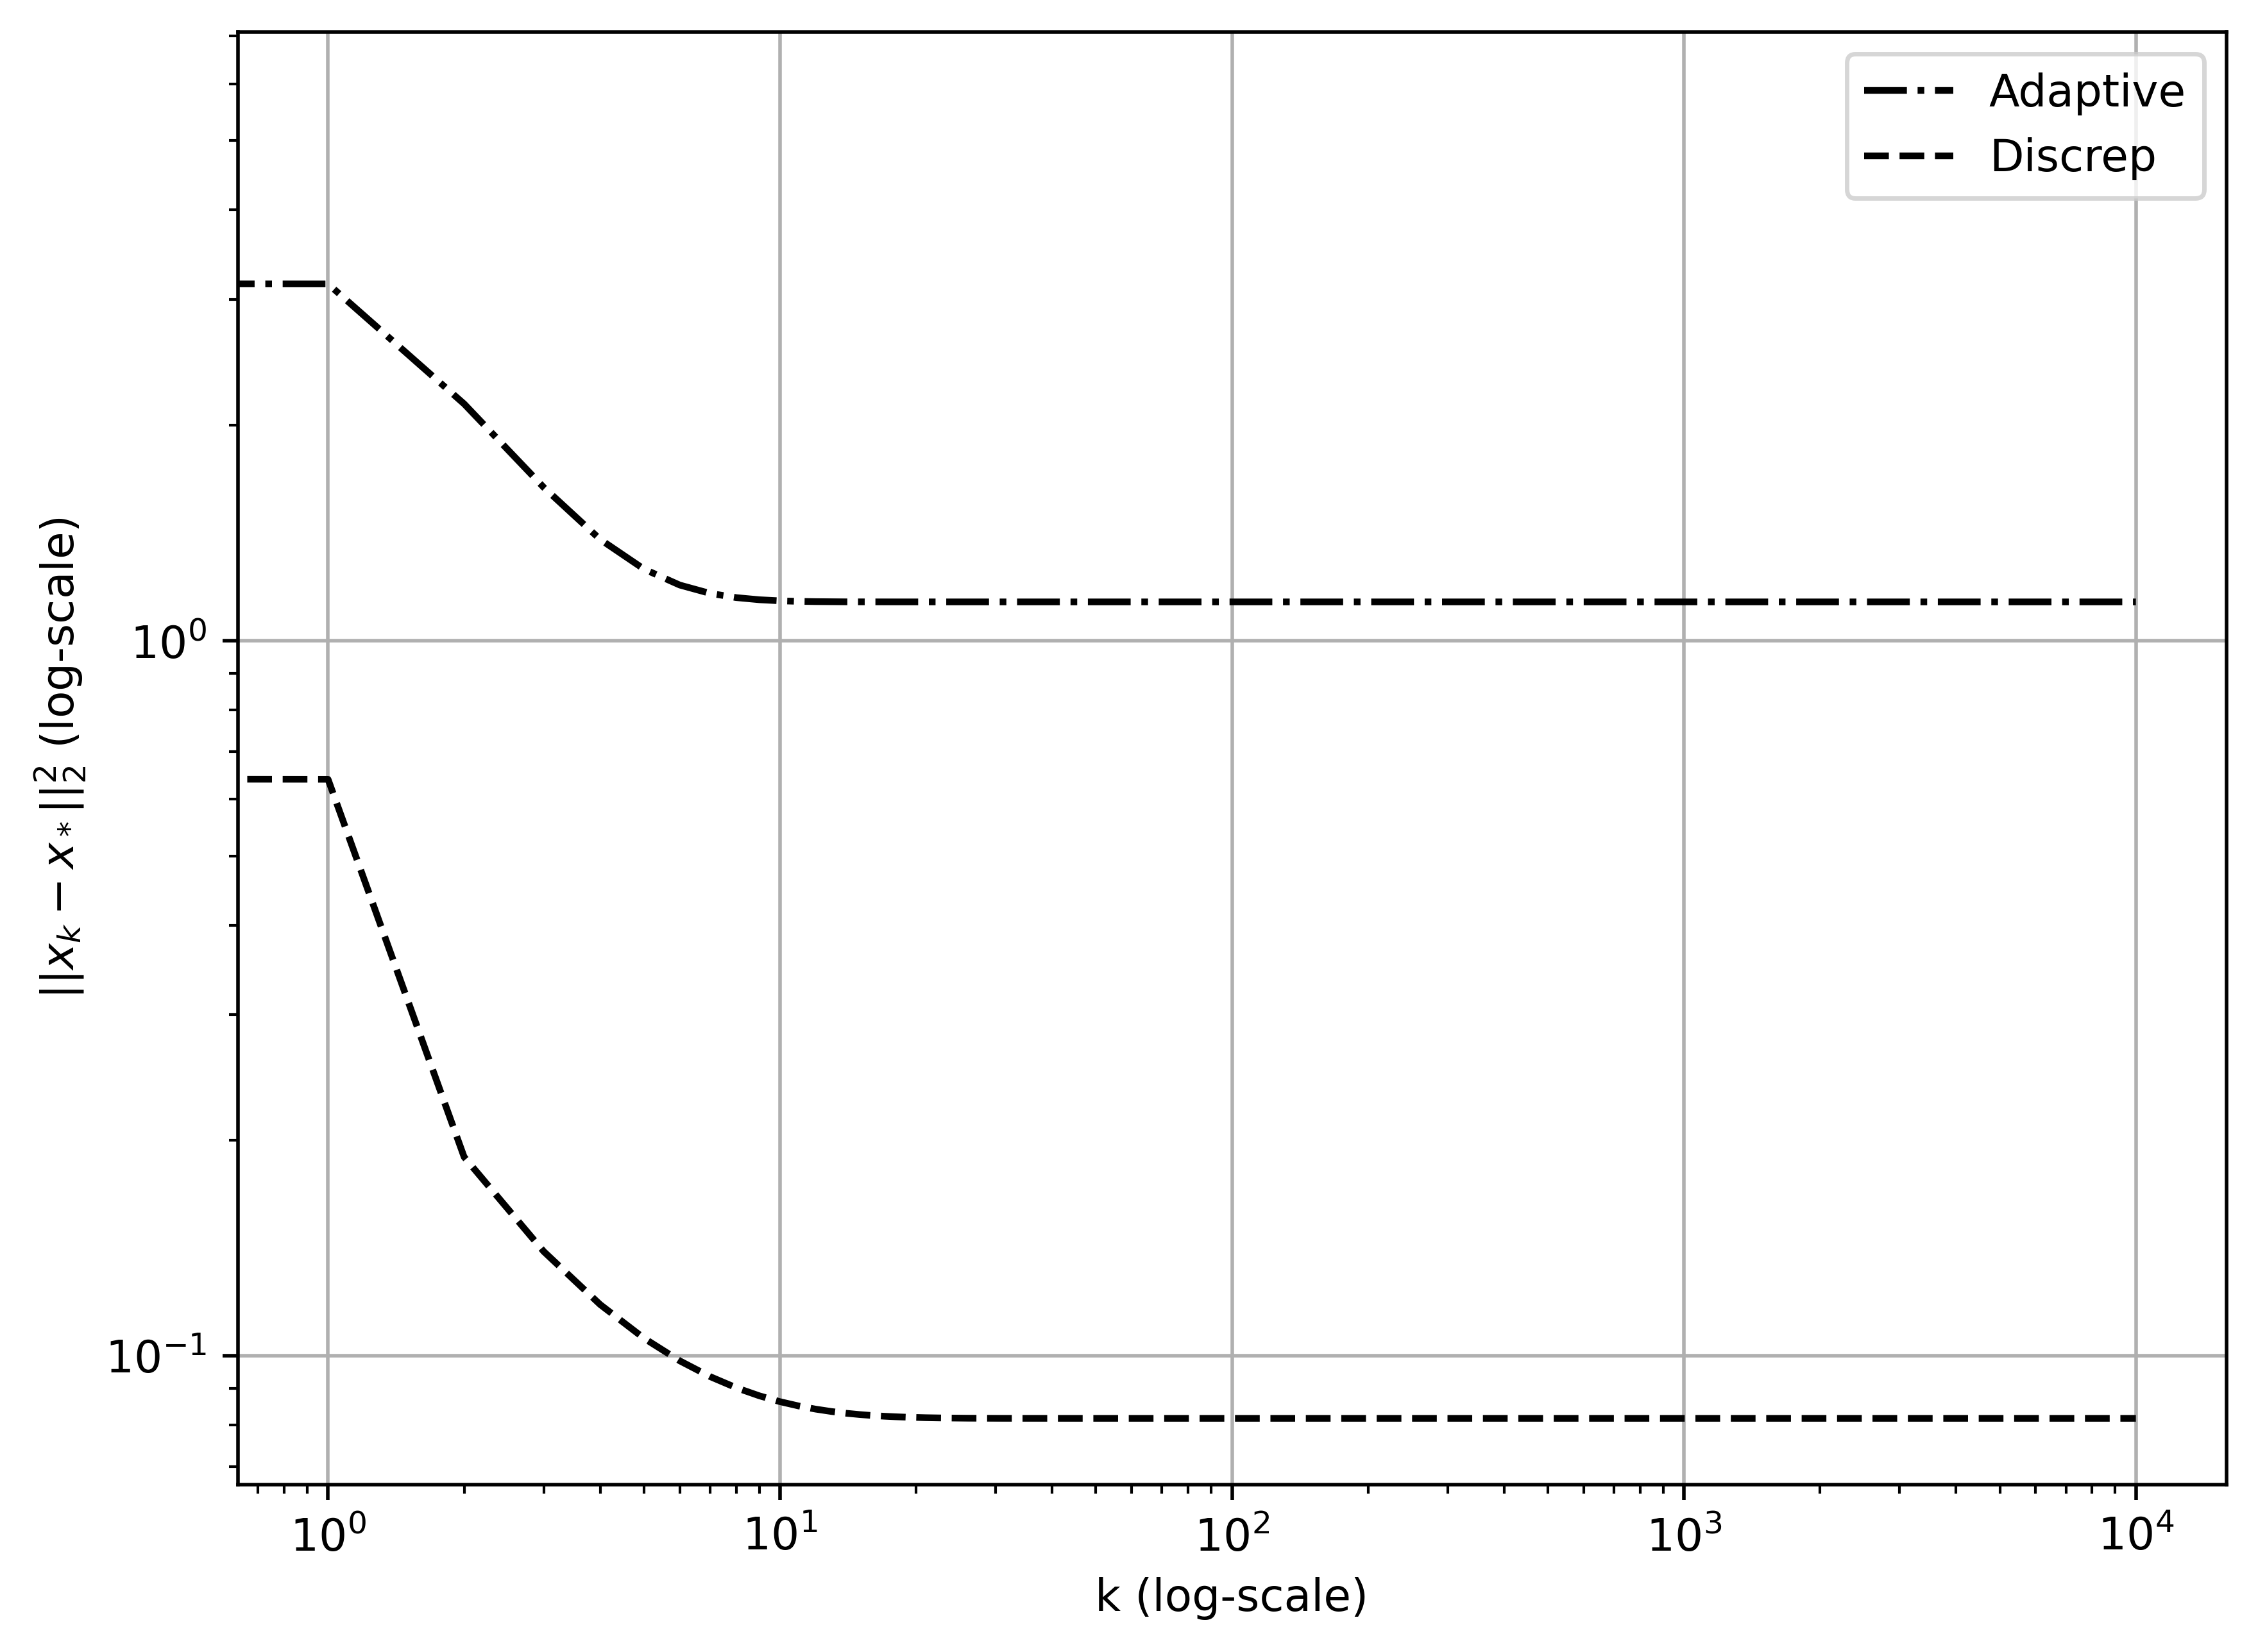
\includegraphics[width=\linewidth]{sharp_convex_x.png}
        \endminipage\hfill
        \minipage{0.49\textwidth}
        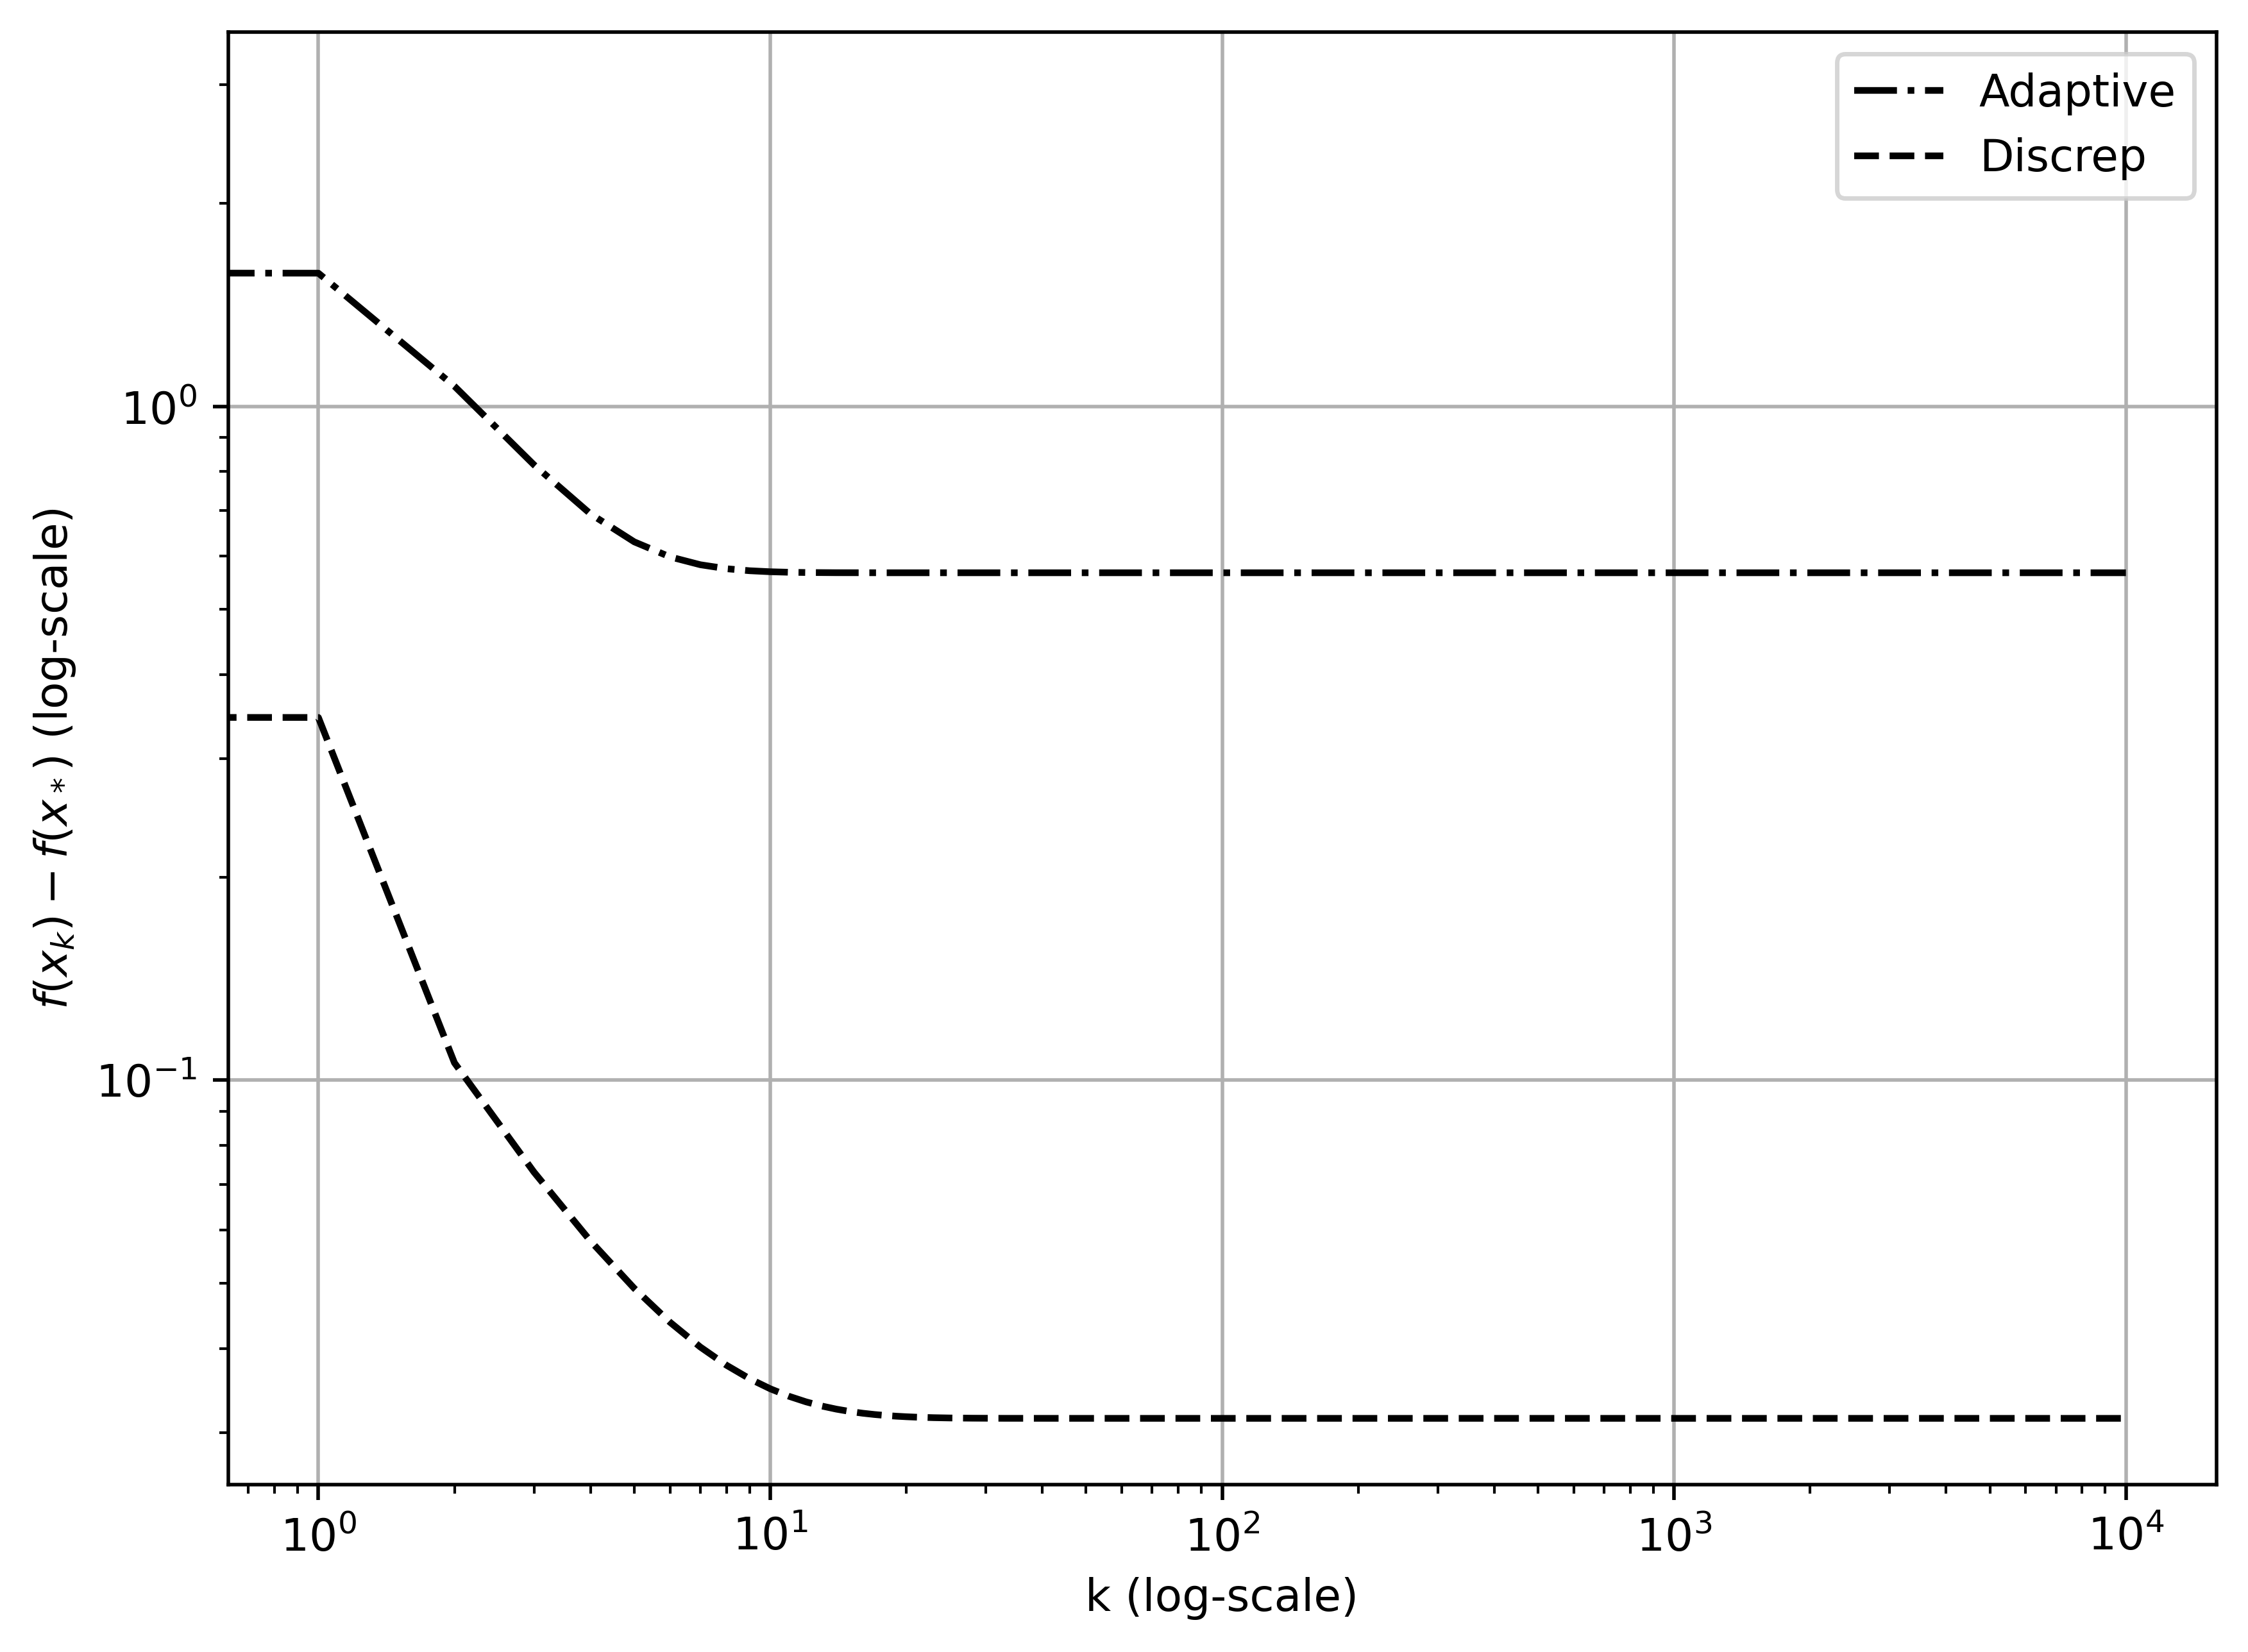
\includegraphics[width=\linewidth]{sharp_convex_f.png}
        \endminipage\hfill
        \caption{ Результаты решения задачи минимизации (\ref{allpha_sphere_cover}), где  $n= 1\,000, r = 0.7525, \alpha = 0.6$.}
        \label{res_sharp_convex}
    \end{figure}

    \begin{figure}[h]
        \minipage{0.49\textwidth}
        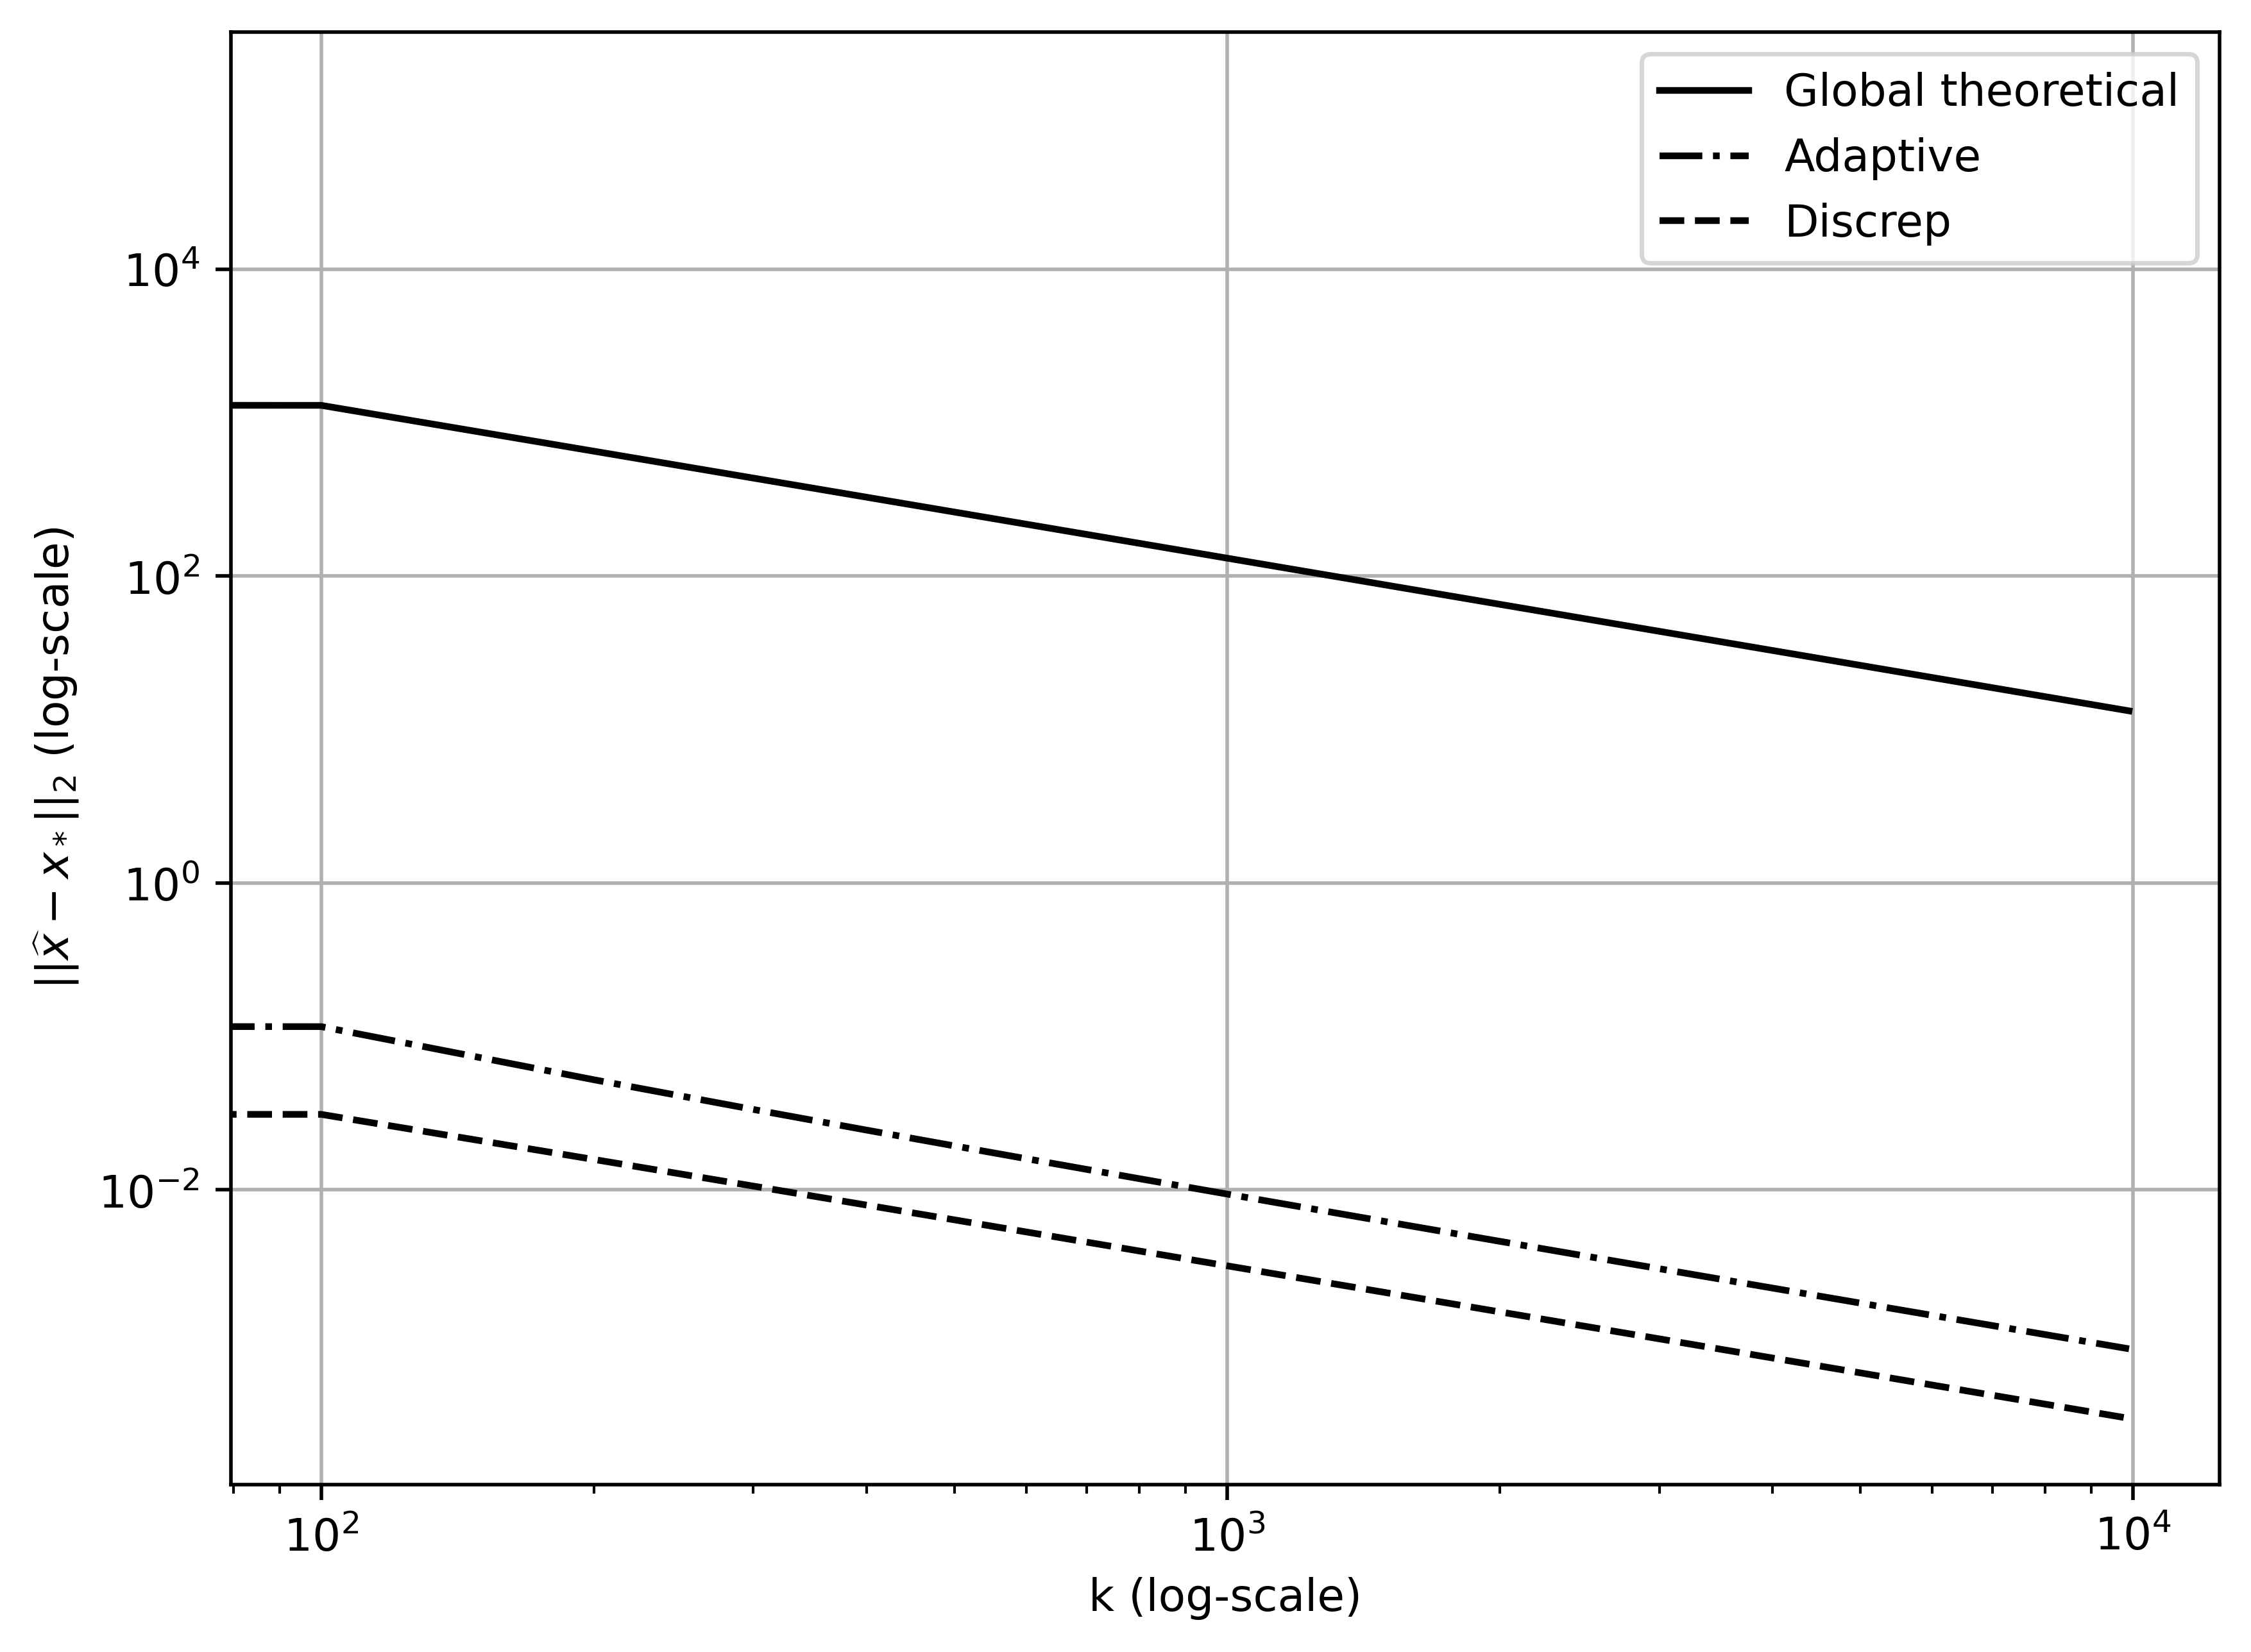
\includegraphics[width=\linewidth]{strong_convex_small_rad_x.png}
        \endminipage\hfill
        \minipage{0.49\textwidth}
        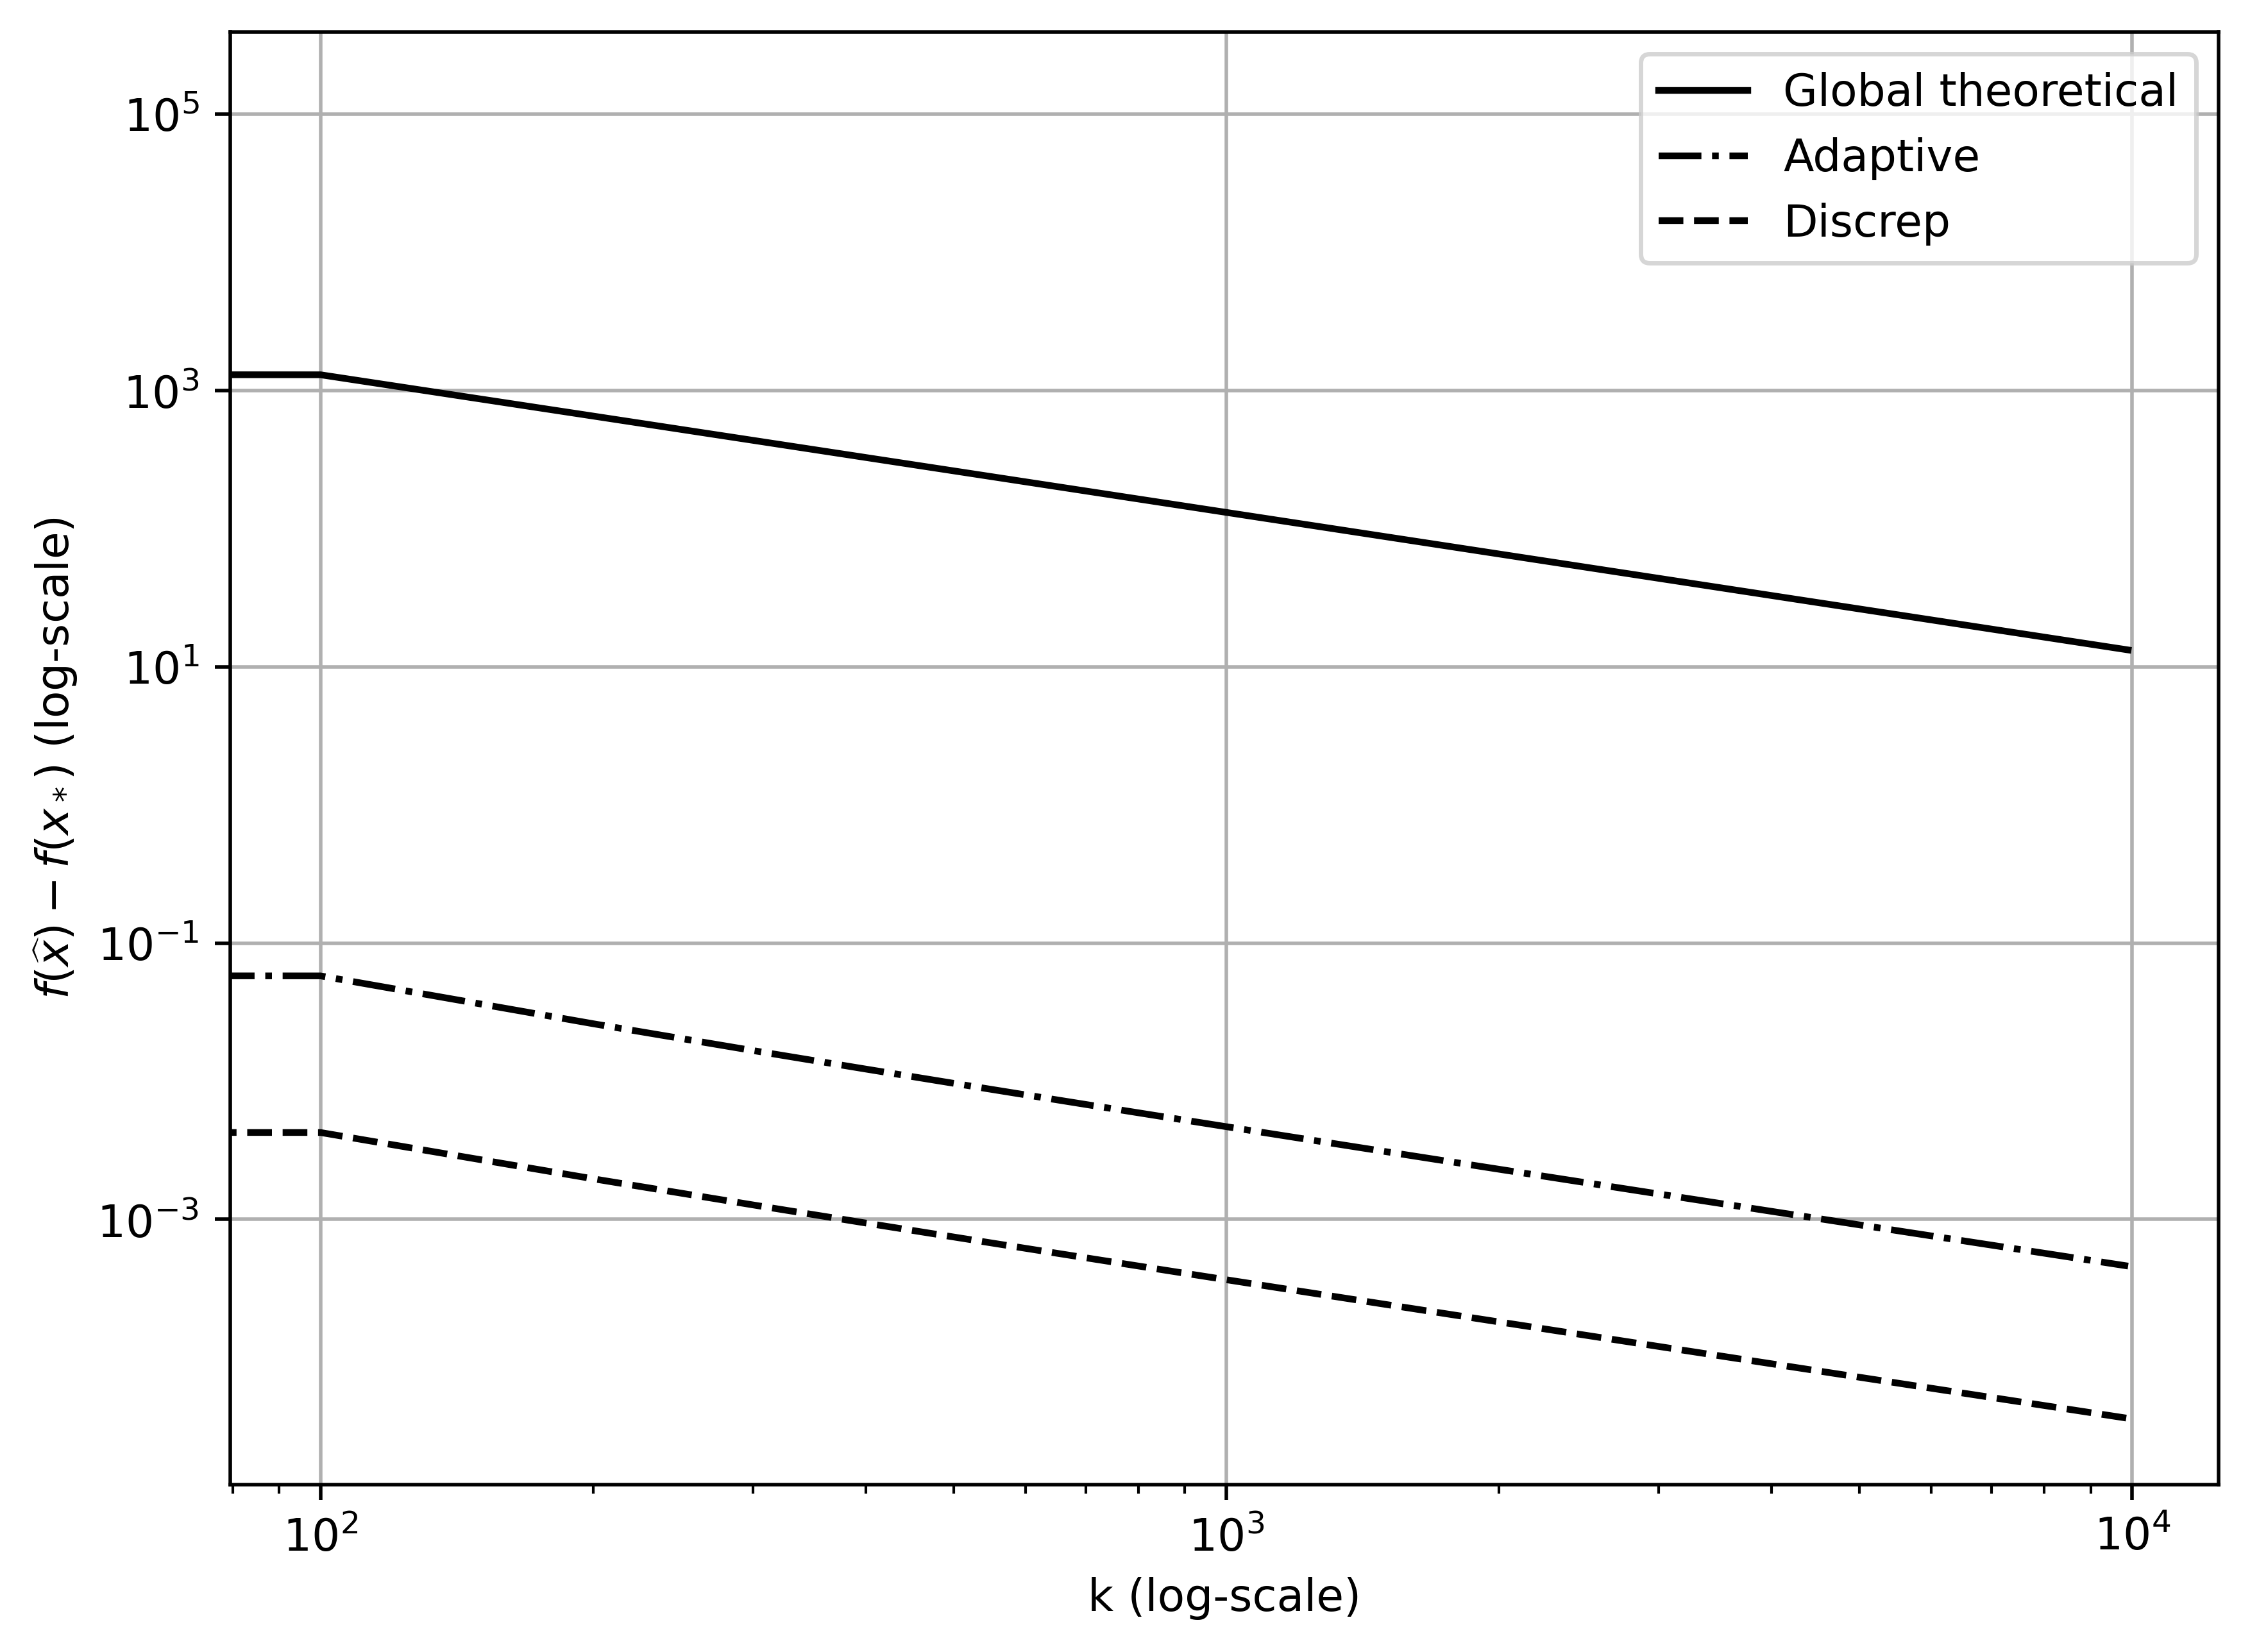
\includegraphics[width=\linewidth]{strong_convex_small_rad_f.png}
        \endminipage\hfill
        \caption{ Результаты решения задачи минимизации (\ref{sphere_cover_strongly}), где  $n= 1\,000, r = 0.7525$.}
        \label{res_strong_convex}
    \end{figure}
\fi
Данные результаты показали потенциальную полезность обоих сравниваемых подходов.


\underline{\textbf{В параграфе 3.3}} вводится аналог условия острого минимума, а именно условие относительного $\gamma$-роста. На его основе к методу классического зеркального спуска применяется схема рестартов, что позволяет улучшить оценки скорости сходимости.

Метод, который будет использоваться для рестартов, был представлен в работе \cite{Lu_2018}:
\begin{theorem} \label{vanilla_mirror} (см. теорему 5 в тексте диссертации)
    Пусть $f$ является выпуклой и относительно $M$-липшицевой на $Q$. Тогда можно задать метод следующим образом:
    \begin{equation} \label{mirr_upd}
        x_{k+1} = \arg \min_{x \in Q} {\left[ f(x_k) + \langle \nabla f(x_k), x - x_k \rangle + \frac{1}{h_k} V(x, x_k)\right]},
    \end{equation}
    где $\{ h_k \}$ - последовательность размеров шагов.
    Для него справедлива следующая оценка скорости сходимости:
    \begin{equation} \label{general_est}
        \min_{0\leq k \leq N} f(x_k) - f(x) \leq \frac{\frac{1}{2} M^2 \sum_{k=0}^N h_k^2 + V(x, x_0)}{\sum_{k=0}^N h_k}
    \end{equation}
\end{theorem}
Введем следующее обозначение
\[
    x_{min}^j  := \argmin_{0\leq k \leq N} f(x_k) \;\;\; \text{на} \;\; j\text{-м рестарте}.
\]
При $j = 0$ имеется ввиду изначальный запуск метода, использующий оригинальную стартовую точку.

\begin{remark} (см. замечание 4 в тексте диссертации)
    Если в \eqref{mirr_upd} в формулировке теоремы \ref{vanilla_mirror} выбрать шаг следующим образом:
    \begin{equation} \label{mirr_step}
        h_{k} = \frac{\sqrt{2 \left[\min\limits_{x_* \in X_*}{V(x_*, x_0)}\right] }}{M\sqrt{N}},
    \end{equation}
    то можно выписать такую оценку скорости сходимости:
    \begin{equation} \label{mirr_est}
        f(x_{min}^0) - f(x_*) \leq \frac{M\sqrt{2 \left[\min\limits_{x_* \in X_*}{V(x_*, x_0)}\right]}}{\sqrt{N}}
    \end{equation}
\end{remark}

Если функция обладает дополнительными свойствами, аналогичными острому минимуму,  то становится возможным применение техники рестартов. Используем аналог данного условия и вслед за Шапиро–Немировским (см. \cite{shapiro_2005} и \cite{shapiro_2021} ) введем условие относительного $\gamma$-роста ($\gamma \geq 1$). Схожее определения вводится в работе \cite{sharp_rest} (см. определение 5.2), однако оно опирается на 1-сильную выпуклость прокс-функции. Вводимое условие относительного $\gamma$-роста позволяет обобщить ряд условий, таких как условия острого минимума, квадратичного доминирования и $\gamma$-роста. 
\begin{definition}
   Будем говорить, что $f$ удовлетворяет условию относительного $\gamma$-роста, если для всякого $x \in Q$ верно неравенство:
   \begin{equation} \label{gamma-growth}
       f(x) - f(x_*) \geq \mu_{\gamma}\left(\min_{x_* \in X_*}{V(x_*,x)}\right)^{\gamma/2},
   \end{equation}
   где $X_*$ --- множество возможный решений задачи минимизации $f$. 
\end{definition}

Справедлива следующая 
\begin{theorem} \label{simple_restart} (см. теорему 6 в тексте диссертации)
    Пусть $f$ удовлетворяет условию относительного $\gamma$-роста \eqref{gamma-growth} и также является относительно $M$-липшицевой на $Q$. В таком случае алгоритм \ref{alg:rest_gamma} после 
    \begin{equation}
    \begin{aligned}
       N =\mathcal{O}\left(\frac{4 M^2}{\mu_{\gamma}^2} \log_2{\left[\frac{\mu_{\gamma}^2}{\varepsilon^2} \left(\min\limits_{x_* \in X_*}{V(x_*, x_0^0)}\right) \right]}\right) \text{ при } \gamma = 1, \\
       N = \mathcal{O}\left(\frac{2^{\gamma + 1} M^2}{2^{(\gamma - 1)} - 1}\left[\frac{1}{\mu_{\gamma}^{\frac{2}{\gamma}}} \varepsilon^{\frac{2(1 - \gamma)}{\gamma}}  - \frac{1}{\mu_{\gamma}^2 \left(\min\limits_{x_* \in X_*}{V(x_*, x_0^0)}\right)^{(\gamma - 1)}} \right]\right) \text{ при } \gamma > 1,
    \end{aligned}
    \end{equation}
    обращений к субградиенту $f$ будет справедливо неравенство
    \begin{equation}
        f(x_{min}^{p-1}) - f(x_*) \leq \varepsilon.
    \end{equation}
\end{theorem}

\begin{algorithm}[htp]
    \caption{Рестарты зеркального спуска при условии относительного $\gamma$-роста.}
    \label{alg:rest_gamma}
    \KwData{$\varepsilon > 0$}
    \KwResult{$x_p$}
    $p \gets 0$\;
    \While{$p < \frac{1}{\gamma} \log_2{\left[\frac{\mu_{\gamma}^2}{\varepsilon^2} \left(\min\limits_{x_* \in X_*}{V(x_*, x_0)}\right)^{\gamma} \right]}$}{
        $x_{p}$ --- результат работы метода \eqref{mirr_upd} с шагом \eqref{mirr_step} и параметром $N_{p} = \ceil*{\frac{2^{\gamma+1} M^2}{\mu_{\gamma}^2 2^{p(1 - \gamma)}} \left(\min\limits_{x_* \in X_*}{V(x_*, x_0)}\right)^{1 - \gamma}}$\;
        $x_0 = x_{min}^p$\;
        $p=p+1$\;
    }
\end{algorithm}


\underline{\textbf{В параграфе 3.4}} предлагается развитие полученных в предыдущем параграфе результатов. На практике для использования приведенной выше теоремы \ref{simple_restart} требуется знание о точном решении для оценки $\min\limits_{x_* \in X_*}{V(x_*, x_0)}$, что лишает данный метод практической пользы. 

Введем $\Theta$ как мажорирующую константу для $\min\limits_{x_* \in X_*}{V(x_*, x_0)}$, что формально описывается
$$
    \Theta^2 \geq \min\limits_{x_* \in X_*}{V(x_*, x_0)}.
$$

Вспомогательный результат, доказанный в данном пункте, позволяет при определении шага следующим образом 
\begin{equation} \label{eps_step}
    h_{k} = \frac{\varepsilon}{\norm{\nabla f(x_k)}^2_*},
\end{equation}
и используя критерий остановки метода
\begin{equation} \label{stop_crit}
    \sum_{k=0}^N \frac{1} {\norm{\nabla f(x_k)}^2_*} \geq \frac{2 \Theta^2}{\varepsilon^2}, \;\;\;\;\text{ где } \Theta^2 \geq \min\limits_{x_* \in X_*}{V(x_*, x_0)},
\end{equation}
получить следующее неравенство для невязки по функции:
\begin{equation} 
\begin{aligned}
    \min_{0\leq k \leq N} f(x_k) - f(x_*) \leq \varepsilon.
\end{aligned}
\end{equation}

\iffalse
    Все вспомогательные результаты, полученные ранее, дают возможность объединить их и сформулировать в виде удобного с практической точки зрения алгоритма. Данный алгоритм требует оценки сверху для расстояния от начальной точки до точного решения, которая может быть сколь угодно <<грубой>>. Это позволяет в дальнейшем усложнять алгоритм, подбирая лучшую начальную оценку расстояния. Также соответствующая теорема \ref{restared_criteria} показывает, что даже существенно <<ослабленная>> версия условия <<острого>> минимума позволяет значимо повысить скорость сходимости.
\fi

Воспользуемся предложенным критерием остановки и сформулируем следующий алгоритм \ref{alg:rest_criteria}. Будем использовать следующее обозначение
\[
    \Theta_0^2 \geq \min\limits_{x_* \in X_*}{V(x_*, x_0)}.
 \]
 \begin{algorithm}[htp]
    \caption{Рестарты зеркального спуска при условии $\gamma$-роста с критерием остановки.}
    \label{alg:rest_criteria}
    \KwData{$\varepsilon > 0$}
    \KwResult{$x_p$}
    $p \gets 0$\;
    $\Theta_0^2 \geq \min\limits_{x_* \in X_*}{V(x_*,x_0)}$\;
    \While{$p < \log_2{\left[\left(\frac{\mu_{\gamma}}{\varepsilon}\right)^{\frac{2}{\gamma}} \Theta_0^2\right]}$}{
        $x_{p}$ --- результат работы метода \eqref{mirr_upd} с шагом \eqref{eps_step} и критерием остановки $\sum_{k=0}^{N_p} \frac{1}{\norm{\nabla f(x_k) }_*^2} \geq \frac{ 2^{(p \gamma - p  + 1)}}{\mu_{\gamma}^2 \Theta_0^{2\gamma - 2} }$, где $N_p$ --- количество итераций на данном рестарте метода\;
        $x_0 = x_{min}^p$\;
        $p=p+1$\;
    }
\end{algorithm}
\begin{theorem} (см. теорему 7 в тексте диссертации)
    Пусть $f$ выпукла и удовлетворяет условию относительного $\gamma$-роста \eqref{gamma-growth} с 1-сильно выпуклой прокс-структурой, а также является $M$-липшицевой на $Q$. В таком случае после работы алгоритма \ref{alg:rest_criteria} будет справедливо неравенство
    \begin{equation}
        f(x_{min}^{p-1}) - f(x_*) \leq \varepsilon.
    \end{equation}
    Для этого потребуется не более чем
    \begin{equation}
        N = \mathcal{O} \left( \frac{4 M^2}{\mu_{\gamma}^2} \log_2{\left[\frac{\mu_{\gamma}^2 \Theta_0^2}{\varepsilon^2} \right]} \right) \text{ при } \gamma = 1
    \end{equation}
    или
    \begin{equation}
        N = \mathcal{O}\left( \frac{2^{(\gamma + 1)} M^2 }{2^{(\gamma - 1)} - 1}\left[ \frac{1}{\mu_{\gamma}^{\frac{2}{\gamma}}} \varepsilon^{\frac{2}{\gamma} - 2} - \frac{1}{\mu_{\gamma}^2 \Theta_0^{2(\gamma - 1)}} \right] \right) \text{ при } \gamma > 1
    \end{equation}
    обращений к оракулу, где $\Theta_0^2$ --- это оценка сверху для $\min\limits_{x_* \in X_*}{V(x_*, x_0)}$.
\end{theorem}

Полученный результат имеет схожие оценки с предыдущей теоремой \ref{simple_restart}, однако на практике критерий остановки может значительно сократить количество итераций, необходимых для достижения заданной точности $\varepsilon$. Также при помощи данного метода легко прогнозируется точность перед каждым рестартом метода, что удобно для контроля за правильностью работы метода. Также подобная информация позволяет переключаться между несколькими модификациями метода, изменяющими, например, параметр $\Theta_0$. Оптимизация данного параметра позволит улучшить оценки без модификации самого метода, что позволит встроить его в более комплексные адаптивные фреймворки в дальнейшем. 

\FloatBarrier
\pdfbookmark{Заключение}{conclusion}                                  % Закладка pdf
В \underline{\textbf{заключении}} приведены основные результаты работы, которые заключаются в следующем:
%% Согласно ГОСТ Р 7.0.11-2011:
%% 5.3.3 В заключении диссертации излагают итоги выполненного исследования, рекомендации, перспективы дальнейшей разработки темы.
%% 9.2.3 В заключении автореферата диссертации излагают итоги данного исследования, рекомендации и перспективы дальнейшей разработки темы.
\begin{enumerate}
  \item Доказаны оптимальные оценки для зеркального спуска для вариационных неравенств с относительно сильно монотонными и относительно ограниченными операторами с точностью до умножения на постоянный множитель.
  \item Получена адаптивная оценка скорости сходимости зеркального спуска для задач минимизации сильно выпуклых функций с использованием локальных аналогов константы Липшица.  
  \item Доказана оценка скорости сходимости рестартованного метода зеркального спуска для относительно липшицевых задач оптимизации с относительным  $\gamma$-ростом.
  \item Предложены адаптивные правила остановки для рестартов исследуемого метода зеркального спуска в предположении липшицевости и 
  $\gamma$-ростом целевой функции и получены теоретические оценки сложности такой  процедуры. 
  \item Проведено исследование и сравнение практической работы методов безградиентного, градиентного и квазинютоновского типов для минимизации функционала OPLS force field, отвечающего за минимизацию энергии белка.
  \item Реализована вспомогательная библиотека для экспериментальной проверки исследуемых в работе субградиентных методов. 
\end{enumerate}


\pdfbookmark{Литература}{bibliography}                                % Закладка pdf


\ifdefmacro{\microtypesetup}{\microtypesetup{protrusion=false}}{} % не рекомендуется применять пакет микротипографики к автоматически генерируемому списку литературы
\urlstyle{rm}                               % ссылки URL обычным шрифтом
\ifnumequal{\value{bibliosel}}{0}{% Встроенная реализация с загрузкой файла через движок bibtex8
    \renewcommand{\bibname}{\large \bibtitleauthor}
    \nocite{*}
    \insertbiblioauthor           % Подключаем Bib-базы
    %\insertbiblioexternal   % !!! bibtex не умеет работать с несколькими библиографиями !!!
}{% Реализация пакетом biblatex через движок biber
    % Цитирования.
    %  * Порядок перечисления определяет порядок в библиографии (только внутри подраздела, если `\insertbiblioauthorgrouped`).
    %  * Если не соблюдать порядок "как для \printbibliography", нумерация в `\insertbiblioauthor` будет кривой.
    %  * Если цитировать каждый источник отдельной командой --- найти некоторые ошибки будет проще.
    \nocite{Stonyakin_2021}%
    \nocite{yakovlev2019algorithms}%
    \nocite{sharp22}%
    \nocite{GorbunovKMR20}%
    %

    \ifnumgreater{\value{usefootcite}}{0}{
        \begin{refcontext}[labelprefix={}]
            \ifnum \value{bibgrouped}>0
                \insertbiblioauthorgrouped    % Вывод всех работ автора, сгруппированных по источникам
            \else
                \insertbiblioauthor      % Вывод всех работ автора
            \fi
        \end{refcontext}
    }{
        \ifnum \totvalue{citeexternal}>0
            \begin{refcontext}[labelprefix=A]
                \ifnum \value{bibgrouped}>0
                    \insertbiblioauthorgrouped    % Вывод всех работ автора, сгруппированных по источникам
                \else
                    \insertbiblioauthor      % Вывод всех работ автора
                \fi
            \end{refcontext}
        \else
            \ifnum \value{bibgrouped}>0
                \insertbiblioauthorgrouped    % Вывод всех работ автора, сгруппированных по источникам
            \else
                \insertbiblioauthor      % Вывод всех работ автора
            \fi
        \fi
        %  \insertbiblioauthorimportant  % Вывод наиболее значимых работ автора (определяется в файле characteristic во второй section)
        \begin{refcontext}[labelprefix={}]
            \insertbiblioexternal            % Вывод списка литературы, на которую ссылались в тексте автореферата
        \end{refcontext}
        % Невидимый библиографический список для подсчёта количества внешних публикаций
        % Используется, чтобы убрать приставку "А" у работ автора, если в автореферате нет
        % цитирований внешних источников.
        \printbibliography[heading=nobibheading, section=0, env=countexternal, keyword=biblioexternal, resetnumbers=true]%
    }
}
\ifdefmacro{\microtypesetup}{\microtypesetup{protrusion=true}}{}
\urlstyle{tt}                               % возвращаем установки шрифта ссылок URL
